\documentclass[12pt,a4paper]{article}
\usepackage[a4paper, margin=0.8in, headheight=14pt]{geometry}
\usepackage{fontspec}
\usepackage{unicode-math}
\setmainfont{TeX Gyre Pagella}
\setmonofont[Scale=0.88]{TeX Gyre Cursor}
\setmathfont{Latin Modern Math}
\usepackage{xcolor}
\usepackage{colortbl}
\usepackage{titlesec}
\usepackage{enumitem}
\usepackage{tabularx}
\usepackage{booktabs}
\usepackage{array}
\usepackage{amsmath}
\usepackage{tikz}
\usetikzlibrary{shapes.geometric, arrows.meta, positioning, calc, fit, decorations.pathreplacing, decorations.pathmorphing}
\usepackage{tcolorbox}
\tcbuselibrary{skins, breakable}
\usepackage{hyperref}
\usepackage{fancyhdr}
\usepackage{graphicx}
\usepackage{microtype}
\hyphenpenalty=10000
\exhyphenpenalty=10000
\sloppy
\usepackage{caption}
\usepackage{setspace}
\usepackage{multirow}
\usepackage{tocloft}
\newcommand{\Q}[1]{\textbf{#1}\par\noindent\ignorespaces}
\definecolor{myred}{RGB}{196,30,58}
\definecolor{mydark}{RGB}{30,30,50}
\definecolor{mygreen}{RGB}{14,120,80}
\definecolor{myteal}{RGB}{0,130,140}
\definecolor{myamber}{RGB}{180,100,0}
\definecolor{mypurple}{RGB}{100,30,160}
\definecolor{mygray}{RGB}{246,247,249}
\definecolor{mgframe}{RGB}{180,185,200}
\definecolor{watermark}{RGB}{145,150,170}
\definecolor{hdrred}{RGB}{250,232,235}
\definecolor{hdrgreen}{RGB}{220,244,233}
\definecolor{hdrteal}{RGB}{220,242,244}
\definecolor{hdramber}{RGB}{253,242,215}
\definecolor{hdrpurple}{RGB}{238,228,255}
\definecolor{hdrgray}{RGB}{238,240,245}
\definecolor{rowalt}{RGB}{250,251,253}

\titleformat{\section}{\large\bfseries\color{myred}}{\thesection.}{0.5em}{}[\vspace{1pt}{\color{myred}\rule{\linewidth}{0.8pt}}]
\titleformat{\subsection}{\normalsize\bfseries\color{myteal}}{\thesubsection}{0.5em}{}
\titlespacing*{\section}{0pt}{18pt}{7pt}
\titlespacing*{\subsection}{0pt}{11pt}{4pt}
\setlength{\parindent}{0pt}
\setlength{\parskip}{4pt}
\renewcommand{\cfttoctitlefont}{\large\bfseries\color{myred}}
\renewcommand{\cftaftertoctitle}{\par\noindent{\color{myred}\rule{\linewidth}{0.8pt}}}
\setlength{\cftbeforetoctitleskip}{0pt}
\setlength{\cftaftertoctitleskip}{6pt}
\renewcommand{\cftsecfont}{\normalsize\bfseries\color{mydark}}
\renewcommand{\cftsecpagefont}{\normalsize\bfseries\color{mydark}}
\renewcommand{\cftsecleader}{\cftdotfill{\cftdotsep}}
\setlength{\cftbeforesecskip}{7pt}
\renewcommand{\cftsubsecfont}{\small\color{mydark}}
\renewcommand{\cftsubsecpagefont}{\small\color{mydark}}
\setlength{\cftbeforesubsecskip}{3pt}
\setlength{\cftsubsecindent}{1.4em}
\renewcommand{\cftpartfont}{\normalsize\bfseries\color{myteal}}
\renewcommand{\cftpartpagefont}{\normalsize\bfseries\color{myteal}}
\setlength{\cftbeforepartskip}{14pt}
\renewcommand{\arraystretch}{1.45}
\setlength{\tabcolsep}{6pt}
\arrayrulecolor{mydark}
\newcolumntype{B}[1]{>{\small\bfseries\raggedright\arraybackslash}m{#1}}
\newcolumntype{C}[1]{>{\centering\arraybackslash}m{#1}}
\newcolumntype{Y}{>{\small\raggedright\arraybackslash}X}
\renewcommand{\tabularxcolumn}[1]{m{#1}}
\newcommand{\currmodule}{Module 1}
\pagestyle{fancy}
\fancyhf{}
\fancyhead[L]{\small\color{myred}\textbf{PE-EC702C}\;\color{mydark}--- Neural Network \& Fuzzy Logic Control}
\fancyhead[R]{\small\color{myteal}\textbf{\currmodule\ Notes}}
\fancyfoot[C]{\small\color{mydark}\thepage}
\fancyfoot[R]{\small\color{watermark}\textit{\copyright\ Biraj}}
\renewcommand{\headrulewidth}{0.5pt}
\renewcommand{\footrulewidth}{0.3pt}

\hypersetup{colorlinks=true, linkcolor=myteal, urlcolor=myteal,
  pdfauthor={Biraj Sarkar},
  pdftitle={PE-EC702C --- Combined Notes}}

\tcbset{
  tikzbox/.style={
    colback=mygray, colframe=mgframe, boxrule=0.6pt, arc=4pt,
    left=8pt, right=8pt, top=6pt, bottom=6pt,
    colbacktitle=mgframe, coltitle=mydark,
    fonttitle=\small\bfseries
  },
  defbox/.style={
    colback=hdrgreen, colframe=mygreen, boxrule=0.8pt, arc=4pt,
    left=9pt, right=9pt, top=6pt, bottom=6pt,
    colbacktitle=mygreen, coltitle=white,
    fonttitle=\small\bfseries
  },
  formulabox/.style={
    colback=hdrteal, colframe=myteal, boxrule=0.8pt, arc=4pt,
    left=9pt, right=9pt, top=7pt, bottom=7pt,
    colbacktitle=myteal, coltitle=white,
    fonttitle=\small\bfseries
  },
  examplebox/.style={
    colback=hdramber, colframe=myamber, boxrule=0.8pt, arc=4pt,
    left=9pt, right=9pt, top=6pt, bottom=6pt,
    colbacktitle=myamber, coltitle=white,
    fonttitle=\small\bfseries,
    breakable
  },
  masonbox/.style={
    colback=hdrpurple, colframe=mypurple, boxrule=0.8pt, arc=4pt,
    left=9pt, right=9pt, top=6pt, bottom=6pt,
    colbacktitle=mypurple, coltitle=white,
    fonttitle=\small\bfseries
  },
  exambox/.style={
    colback=hdrpurple, colframe=mypurple, boxrule=1pt, arc=5pt,
    left=10pt, right=10pt, top=8pt, bottom=8pt,
    colbacktitle=mypurple, coltitle=white,
    fonttitle=\bfseries,
    breakable, title after break={\textbf{Frequently Asked / Viva Questions (contd.)}}}
}
\tcbset{after={\color{black}}}

\tikzset{
  block/.style={rectangle, draw=myteal, fill=hdrteal,
    text width=2.2cm, align=center, minimum height=0.85cm,
    font=\small, rounded corners=3pt, line width=0.7pt},
  arrow/.style={-Stealth, thick, color=mydark},
  line/.style={thick, color=mydark}
}

\newcommand{\modulestart}[2]{%
  \clearpage
  \renewcommand{\currmodule}{Module #1}%
  \phantomsection
  \addcontentsline{toc}{part}{Module #1: #2}%
  \setcounter{section}{0}%
  \begin{center}
    \vspace*{1.0cm}
    {\Huge\bfseries\color{myred} Module #1}\\[10pt]
    {\Large\bfseries\color{mydark} #2}\\[10pt]
    {\color{myred}\rule{0.55\linewidth}{1.2pt}}
  \end{center}
  \vspace{14pt}
}
\begin{document}

\thispagestyle{empty}
\vspace*{1.0cm}
\begin{center}
  {\Huge\bfseries\color{myred} PE-EC702C}\\[10pt]
  {\LARGE\bfseries\color{mydark} Neural Network \& Fuzzy Logic Control}\\[20pt]
  {\color{myred}\rule{0.7\linewidth}{1.5pt}}\\[18pt]
  {\Large\color{myteal}\textbf{Combined Module Notes}}\\[8pt]
  {\large\color{mydark} Modules 1 -- 5}\\[40pt]
  {\normalsize\color{mydark} Semester VII \quad$\bullet$\quad 3L:0T:0P \quad$\bullet$\quad 3 Credits}\\[12pt]
  {\normalsize\color{mydark} CGEC \;$|$\; B.Tech ECE (2023--27)}\\[6pt]
  {\normalsize\color{mydark}\textit{Biraj Sarkar}}
\end{center}
\vspace{1.0cm}
\begin{center}
  \begin{tcolorbox}[colback=mygray, colframe=mgframe, boxrule=0.5pt, arc=3pt, width=0.85\linewidth]
    \centering\small\color{mydark}
    \textbf{Disclaimer / Study Guide Notice:}\\
    These are condensed \textbf{Short Notes} focusing on core theory, key formulas, block/circuit diagrams, and standard viva Q\&As for university exam revision. Exhaustive numerical practice problems and derivation edge cases are not covered. This serves as a quick-revision reference guide for students.
  \end{tcolorbox}
\end{center}
\vfill
\begin{center}{\small\color{watermark}\textit{Exam-Ready Notes}}\end{center}
\clearpage

\hypersetup{linkcolor=mydark}
\tableofcontents
\hypersetup{linkcolor=myteal}
\clearpage

% -- Module 1 -----------------------------------------------------------------
\modulestart{1}{Biological vs. Artificial Neural Networks}

\section{Biological vs. Artificial Neural Networks}
% ===============================================================================

An Artificial Neural Network (ANN) is an information-processing paradigm inspired by the structure and functional aspects of biological neural systems.

\begin{tcolorbox}[defbox, title={Artificial Neural Network (ANN)}]
An \textbf{Artificial Neural Network (ANN)} is a parallel, distributed computational model consisting of simple processing units (neurons) interconnected by weighted links, designed to learn patterns and relationships from data.
\end{tcolorbox}

\subsection{Structural and Functional Mapping}
The biological brain consists of billions of highly interconnected cells called neurons. The artificial neuron models this biological mechanism:

\begin{tcolorbox}[tikzbox, title={Biological vs. Artificial Neuron Mapping}]
\centering
\begin{minipage}{0.48\textwidth}
  \centering
  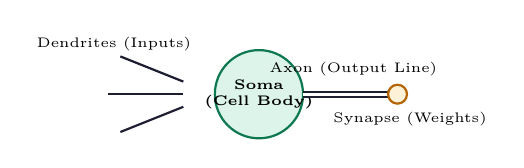
\begin{tikzpicture}[scale=0.8, every node/.style={font=\tiny}]
    % Dendrites
    \draw[thick, color=mydark] (-2.2, 0.6) -- (-1.2, 0.2);
    \draw[thick, color=mydark] (-2.2, -0.6) -- (-1.2, -0.2);
    \draw[thick, color=mydark] (-2.4, 0) -- (-1.2, 0);
    \node at (-2.3, 0.8) {Dendrites (Inputs)};
    
    % Soma
    \draw[thick, fill=hdrgreen, draw=mygreen] (0,0) circle (0.7cm);
    \node[align=center] at (0,0) {\textbf{Soma}\\\textbf{(Cell Body)}};
    
    % Axon
    \draw[line, double, double distance=1pt] (0.7, 0) -- (2.2, 0);
    \node at (1.5, 0.4) {Axon (Output Line)};
    
    % Synapse
    \draw[thick, fill=hdramber, draw=myamber] (2.2, 0) circle (0.15cm);
    \node at (2.4, -0.4) {Synapse (Weights)};
  \end{tikzpicture}
  \par\vspace{2pt}\small\textbf{Biological Neuron Elements}
\end{minipage}
\hfill
\begin{minipage}{0.48\textwidth}
  \centering
  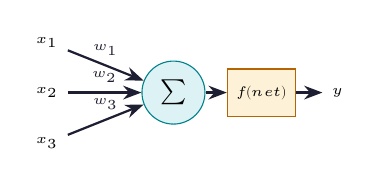
\begin{tikzpicture}[scale=0.8, every node/.style={font=\tiny}]
    % Inputs
    \node (x1) at (-2.0, 0.8) {$x_1$};
    \node (x2) at (-2.0, 0) {$x_2$};
    \node (x3) at (-2.0, -0.8) {$x_3$};
    
    % Summing junction
    \node[circle, draw=myteal, fill=hdrteal, minimum size=0.8cm, font=\small] (sum) at (0,0) {$\sum$};
    
    % Weights
    \draw[arrow] (x1) -- node[midway, above] {$w_1$} (sum);
    \draw[arrow] (x2) -- node[midway, above] {$w_2$} (sum);
    \draw[arrow] (x3) -- node[midway, above] {$w_3$} (sum);
    
    % Activation
    \node[rectangle, draw=myamber, fill=hdramber, minimum height=0.6cm, minimum width=0.8cm] (act) at (1.4, 0) {$f(net)$};
    \draw[arrow] (sum) -- (act);
    
    % Output
    \node (y) at (2.6, 0) {$y$};
    \draw[arrow] (act) -- (y);
  \end{tikzpicture}
  \par\vspace{2pt}\small\textbf{Artificial Neuron Model}
\end{minipage}
\end{tcolorbox}

\par\noindent
The physical correspondences between biological and artificial components are summarized below:
\par\noindent
{\renewcommand{\arraystretch}{1.9}%
\begin{tabularx}{\linewidth}{|>{\bfseries}B{3.5cm}|Y|Y|}
\hline
Biological Component & Artificial Equivalent & Functional Role \\
\hline
Dendrites & Inputs ($x_i$) & Receives signals from other neurons \\[4pt]
\hline
Soma (Cell Body) & Summing Junction ($\sum$) & Aggregates all incoming weighted inputs \\[6pt]
\hline
Axon & Output Transmission Line & Carries the output activation signal \\
\hline
Synapse & Weights ($w_i$) & Regulates the strength of connections \\[4pt]
\hline
Synaptic Threshold & Activation Function ($f$) & Determines output state based on total input \\
\hline
\end{tabularx}}

% ===============================================================================
\section{Typical Architectures of ANNs}
% ===============================================================================

Neural network topologies are broadly classified into three categories based on the flow of signals and feedback loops:

\begin{enumerate}[leftmargin=*, itemsep=4pt]
  \item \textbf{Single-Layer Feedforward Network:} Consists of an input layer of source nodes that connects directly to an output layer of neurons. There are no feedback loops and no hidden layers. (Example: Hebb net, Perceptron, Adaline).
  \item \textbf{Multi-Layer Feedforward Network:} Contains one or more hidden layers of processing units between the input and output layers. This architecture enables the network to learn non-linear decision boundaries. (Example: Backpropagation MLP).
  \item \textbf{Recurrent (Feedback) Network:} Contains at least one feedback loop where output signals are fed back as inputs to neurons in previous or current layers. (Example: Hopfield Network, BAM).
\end{enumerate}

% ===============================================================================
\section{Common Activation Functions}
% ===============================================================================

Activation functions (transfer functions) introduce non-linearity into the neuron model, allowing it to solve complex, non-linear problems.

\begin{tcolorbox}[formulabox, title={Mathematical Formulations of Activation Functions}]
Let $net = \sum w_i x_i + b$ be the net input to the neuron.
\par\vspace{4pt}
{\renewcommand{\arraystretch}{1.9}%
\begin{tabularx}{\linewidth}{B{3.2cm} Y B{3.8cm}}
\hline
Function & Mathematical Form & Range \\[4pt]
\hline
Binary Step & $f(net) = \begin{cases} 1 & \text{if } net \ge 0 \\ 0 & \text{if } net < 0 \end{cases}$ & $\{0, 1\}$ \\[8pt]
\hline
Bipolar Step & $f(net) = \begin{cases} 1 & \text{if } net \ge 0 \\ -1 & \text{if } net < 0 \end{cases}$ & $\{-1, 1\}$ \\[8pt]
\hline
Binary Sigmoid & $f(net) = \frac{1}{1 + e^{-\lambda net}}$ & $(0, 1)$ \\[6pt]
\hline
Bipolar Sigmoid & $f(net) = \frac{2}{1 + e^{-\lambda net}} - 1 = \tanh\left(\frac{\lambda net}{2}\right)$ & $(-1, 1)$ \\[6pt]
\hline
Rectified Linear (ReLU) & $f(net) = \max(0, net)$ & $[0, \infty)$ \\[4pt]
\hline
\end{tabularx}}
\end{tcolorbox}

\begin{tcolorbox}[tikzbox, title={Activation Function Shapes}]
\centering
\begin{minipage}{0.23\textwidth}
  \centering
  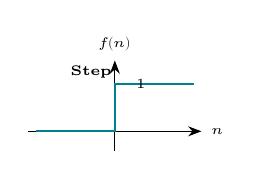
\begin{tikzpicture}[scale=0.5]
    \draw[-Stealth] (-2.2,0) -- (2.2,0) node[right] {\tiny $n$};
    \draw[-Stealth] (0,-0.5) -- (0,1.8) node[above] {\tiny $f(n)$};
    \draw[thick, color=myteal] (-2.0, 0) -- (0, 0) -- (0, 1.2) -- (2.0, 1.2);
    \node at (0.3, 1.2) [right] {\tiny $1$};
    \node at (-0.6, 1.5) {\textbf{\tiny Step}};
  \end{tikzpicture}
\end{minipage}
\hfill
\begin{minipage}{0.23\textwidth}
  \centering
  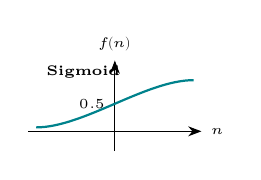
\begin{tikzpicture}[scale=0.5]
    \draw[-Stealth] (-2.2,0) -- (2.2,0) node[right] {\tiny $n$};
    \draw[-Stealth] (0,-0.5) -- (0,1.8) node[above] {\tiny $f(n)$};
    \draw[thick, color=myteal] (-2.0, 0.1) .. controls (-0.8, 0.1) and (0.8, 1.3) .. (2.0, 1.3);
    \node at (0, 0.7) [left] {\tiny $0.5$};
    \node at (-0.8, 1.5) {\textbf{\tiny Sigmoid}};
  \end{tikzpicture}
\end{minipage}
\hfill
\begin{minipage}{0.23\textwidth}
  \centering
  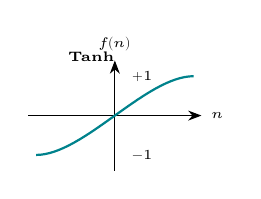
\begin{tikzpicture}[scale=0.5]
    \draw[-Stealth] (-2.2,0) -- (2.2,0) node[right] {\tiny $n$};
    \draw[-Stealth] (0,-1.4) -- (0,1.4) node[above] {\tiny $f(n)$};
    \draw[thick, color=myteal] (-2.0, -1.0) .. controls (-0.8, -1.0) and (0.8, 1.0) .. (2.0, 1.0);
    \node at (0.2, 1.0) [right] {\tiny $+1$};
    \node at (0.2, -1.0) [right] {\tiny $-1$};
    \node at (-0.6, 1.5) {\textbf{\tiny Tanh}};
  \end{tikzpicture}
\end{minipage}
\hfill
\begin{minipage}{0.23\textwidth}
  \centering
  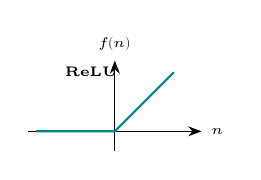
\begin{tikzpicture}[scale=0.5]
    \draw[-Stealth] (-2.2,0) -- (2.2,0) node[right] {\tiny $n$};
    \draw[-Stealth] (0,-0.5) -- (0,1.8) node[above] {\tiny $f(n)$};
    \draw[thick, color=myteal] (-2.0, 0) -- (0, 0) -- (1.5, 1.5);
    \node at (-0.6, 1.5) {\textbf{\tiny ReLU}};
  \end{tikzpicture}
\end{minipage}
\end{tcolorbox}

% ===============================================================================
\section{McCulloch-Pitts Neuron Model}
% ===============================================================================

The McCulloch-Pitts (M-P) neuron, introduced in 1943, was the first mathematical model of an artificial neuron.

\begin{tcolorbox}[defbox, title={McCulloch-Pitts Neuron}]
An \textbf{M-P Neuron} is a binary threshold device where inputs are either $0$ or $1$, weights are fixed integers (usually $+1$ for excitatory and $-1$ for inhibitory), and the output is determined by comparing the weighted sum against a threshold $\theta$.
\end{tcolorbox}

\subsection{Mathematical Formulation}
The activation of an M-P neuron is governed by:
\begin{equation}
  y = f(net) = \begin{cases} 1 & \text{if } net \ge \theta \\ 0 & \text{if } net < \theta \end{cases}
\end{equation}
where the net input $net$ is computed as:
\begin{equation}
  net = \sum_{i=1}^n w_i x_i
\end{equation}
\textbf{Inhibitory Rule:} If any inhibitory input $x_j$ is active (i.e. $x_j = 1$ where $w_j = -1$ or $-\infty$), the output $y$ is forced to $0$ immediately, regardless of the excitatory sum.

\subsection{Linear Separability and the XOR Problem}
A classification problem is \textbf{linearly separable} if a single straight line (in 2D), plane (in 3D), or hyperplane (in higher dimensions) can completely separate the output classes.
\par\noindent
Simple logic gates like AND, OR, and NOT are linearly separable. However, the XOR (Exclusive OR) gate is \textbf{not} linearly separable, as a single line cannot separate the outputs $\{0\}$ and $\{1\}$. This limitation led to the development of multi-layer neural networks.

\begin{tcolorbox}[tikzbox, title={Linear Separability of AND vs. XOR}]
\centering
\begin{minipage}{0.48\textwidth}
  \centering
  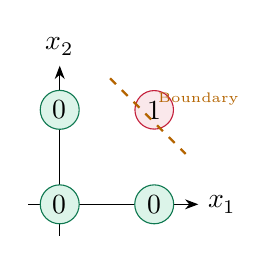
\begin{tikzpicture}[scale=0.8]
    \draw[-Stealth] (-0.5,0) -- (2.2,0) node[right] {$x_1$};
    \draw[-Stealth] (0,-0.5) -- (0,2.2) node[above] {$x_2$};
    \node[circle, draw=mygreen, fill=hdrgreen, inner sep=2pt] at (0,0) {$0$};
    \node[circle, draw=mygreen, fill=hdrgreen, inner sep=2pt] at (1.5,0) {$0$};
    \node[circle, draw=mygreen, fill=hdrgreen, inner sep=2pt] at (0,1.5) {$0$};
    \node[circle, draw=myred, fill=hdrred, inner sep=2pt] at (1.5,1.5) {$1$};
    \draw[dashed, thick, color=myamber] (0.8, 2.0) -- (2.0, 0.8) node[midway, above right] {\tiny Boundary};
  \end{tikzpicture}
  \par\vspace{2pt}\small\textbf{AND Gate (Linearly Separable)}
\end{minipage}
\hfill
\begin{minipage}{0.48\textwidth}
  \centering
  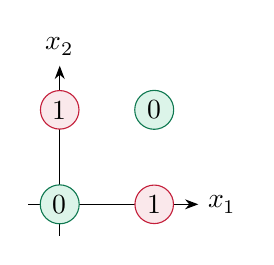
\begin{tikzpicture}[scale=0.8]
    \draw[-Stealth] (-0.5,0) -- (2.2,0) node[right] {$x_1$};
    \draw[-Stealth] (0,-0.5) -- (0,2.2) node[above] {$x_2$};
    \node[circle, draw=mygreen, fill=hdrgreen, inner sep=2pt] at (0,0) {$0$};
    \node[circle, draw=myred, fill=hdrred, inner sep=2pt] at (1.5,0) {$1$};
    \node[circle, draw=myred, fill=hdrred, inner sep=2pt] at (0,1.5) {$1$};
    \node[circle, draw=mygreen, fill=hdrgreen, inner sep=2pt] at (1.5,1.5) {$0$};
  \end{tikzpicture}
  \par\vspace{2pt}\small\textbf{XOR Gate (Non-Linearly Separable)}
\end{minipage}
\end{tcolorbox}

% ===============================================================================
\section{Hebb Net Learning Rule}
% ===============================================================================

Proposed by Donald Hebb in 1949, this is the oldest learning algorithm. It is based on the biological premise: *"Neurons that fire together, wire together."*

\begin{tcolorbox}[defbox, title={Hebbian Learning Rule}]
If two connected neurons are active simultaneously, the weight of the connection between them should be increased:
\begin{equation}
  w_i(\text{new}) = w_i(\text{old}) + x_i y
\end{equation}
where $x_i$ is the input and $y$ is the output.
\end{tcolorbox}

\subsection{Hebb Net Training Algorithm}
\begin{enumerate}[leftmargin=*, itemsep=2.5pt]
  \item Initialize all weights $w_i = 0$ and bias $b = 0$.
  \item For each training input vector $s = (s_1, s_2, \ldots, s_n)$ and target output $t$:
    \begin{itemize}[leftmargin=1.5em, itemsep=1.5pt]
      \item Set activation of input units $x_i = s_i$.
      \item Set activation of output unit $y = t$.
      \item Update weights: $w_i(\text{new}) = w_i(\text{old}) + x_i y$.
      \item Update bias: $b(\text{new}) = b(\text{old}) + y$.
    \end{itemize}
\end{enumerate}
\textit{Note: Hebb net learning works best when inputs and targets are represented in bipolar form ($\{-1, 1\}$) rather than binary form ($\{0, 1\}$).}

% ===============================================================================
\section{Perceptron Learning Algorithm}
% ===============================================================================

Developed by Frank Rosenblatt in 1958, the Perceptron is a supervised learning model used for binary classification.

\begin{tcolorbox}[formulabox, title={Perceptron Activation \& Weight Update}]
The output is computed using a binary/bipolar step activation:
\begin{equation}
  y = \begin{cases} 1 & \text{if } \sum w_i x_i + b \ge \theta \\ -1/0 & \text{if } \sum w_i x_i + b < \theta \end{cases}
\end{equation}
If the computed output $y$ does not match the target $t$, the weights and bias are updated using the Perceptron Learning Rule:
\begin{equation}
  w_i(\text{new}) = w_i(\text{old}) + \alpha (t - y) x_i
\end{equation}
\begin{equation}
  b(\text{new}) = b(\text{old}) + \alpha (t - y)
\end{equation}
where $\alpha \in (0, 1]$ is the learning rate.
\end{tcolorbox}

% ===============================================================================
\section{Adaline and Madaline Networks}
% ===============================================================================

\subsection{Adaline (Adaptive Linear Neuron)}
Developed by Widrow and Hoff (1960), Adaline is a single-element network that utilizes the Delta Rule (LMS - Least Mean Squares) for training.

\begin{tcolorbox}[defbox, title={Adaline vs. Perceptron}]
Unlike the Perceptron where weights are updated based on the thresholded binary output, Adaline updates weights using the continuous analog output \textbf{before} the activation function is applied.
\end{tcolorbox}

\par\noindent
The weight update in Adaline minimizes the mean squared error (gradient descent):
\begin{equation}
  w_i(\text{new}) = w_i(\text{old}) + \alpha (t - net) x_i
\end{equation}
where $net = \sum w_i x_i + b$ is the analog pre-activation sum.

\subsection{Madaline (Many Adalines)}
Madaline consists of a multilayer organization of Adaline units. The input layer connects to a hidden layer of Adaline units, which in turn connect to Madaline output units using fixed logic functions (AND, OR, or Majority vote). Madaline is trained using MRI (Madaline Rule I) or MRII algorithms.

% ===============================================================================
\section{Pattern Association Networks}
% ===============================================================================

Pattern association involves storing set of pattern pairs $(s^p, t^p)$ such that when an input pattern $s^p$ is presented, the network recalls the associated target pattern $t^p$.

\subsection{Classification of Associative Memories}
\begin{enumerate}[leftmargin=*, itemsep=3.5pt]
  \item \textbf{Auto-Associative Net:}
    A network where the input vector and target vector are identical ($s^p = t^p$). Its primary goal is pattern retrieval, denoising, or pattern completion. If a distorted or incomplete version of pattern $s^p$ is presented, the network outputs the original stored pattern $s^p$.
  \item \textbf{Hetero-Associative Net:}
    A network where the input vector and target vector are different ($s^p \neq t^p$, and they may reside in spaces of different dimensions). It maps an input vector in space $X$ to an associated target vector in space $Y$.
  \item \textbf{Iterative Auto-Associative Net:}
    A recurrent auto-associative network where output states are fed back as inputs dynamically. The network iteratively updates its activation values until it settles (converges) into a stable state representing one of the stored patterns (e.g., Hopfield networks).
\end{enumerate}

\subsection{Training Rules for Pattern Association}
Training an associative memory network involves constructing a weight matrix $W$ to map inputs to targets:
\begin{enumerate}[leftmargin=*, itemsep=3.5pt]
  \item \textbf{Hebbian Learning Rule (Outer Product Rule):}
    For $P$ bipolar pattern pairs $(s^p, t^p)$ where $s^p \in \{-1, 1\}^n$ and $t^p \in \{-1, 1\}^m$, the weight matrix is formed by summing the outer products of input-target pairs:
    \begin{equation}
      W = \sum_{p=1}^P (s^p)^T t^p \quad \implies \quad w_{ij} = \sum_{p=1}^P s_i^p t_j^p
    \end{equation}
  \item \textbf{Delta Rule (LMS / Widrow-Hoff Rule):}
    Used when patterns are not orthogonally separable. It is an iterative gradient descent rule that updates weights based on output error to minimize mean squared error:
    \begin{equation}
      \Delta w_{ij} = \alpha (t_j^p - y_j^p) s_i^p
    \end{equation}
    where $\alpha$ is the learning rate, $t_j^p$ is the target, and $y_j^p$ is the actual output.
\end{enumerate}

% ===============================================================================
\section{Bidirectional Associative Memory (BAM)}
% ===============================================================================

Introduced by Bart Kosko in 1988, BAM is a hetero-associative recurrent network that maps input vectors from space $X$ to target vectors in space $Y$.

\begin{tcolorbox}[formulabox, title={BAM Weight Matrix and Recall}]
Given $P$ bipolar pattern pairs $(S^p, T^p)$ where $S^p \in \{-1,1\}^n$ and $T^p \in \{-1,1\}^m$:
\par\noindent
The weight correlation matrix $W$ of size $n \times m$ is computed as:
\begin{equation}
  W = \sum_{p=1}^P (S^p)^T T^p
\end{equation}
\par\noindent
\textbf{Bidirectional Recall Process:}
\begin{itemize}[leftmargin=*, itemsep=3pt]
  \item \textbf{Forward Direction:} Feed input vector $X$ to recall output $Y$:
    \begin{equation}
      y_j = \text{sign}\left( \sum_{i=1}^n x_i w_{ij} \right) \quad \rightarrow \quad Y = \text{sign}(X W)
    \end{equation}
  \item \textbf{Backward Direction:} Feed output vector $Y$ back to recall input $X$:
    \begin{equation}
      x_i = \text{sign}\left( \sum_{j=1}^m y_j w_{ij} \right) \quad \rightarrow \quad X = \text{sign}(Y W^T)
    \end{equation}
\end{itemize}
\end{tcolorbox}

% ===============================================================================
\section{Worked Examples}
% ===============================================================================

\begin{tcolorbox}[examplebox, title={McCulloch-Pitts AND gate Implementation}]
\textbf{Problem:} Implement an AND gate using a McCulloch-Pitts neuron with binary inputs $x_1, x_2 \in \{0, 1\}$. Determine the weights and threshold $\theta$.
\par\vspace{4pt}\noindent\rule{\linewidth}{0.5pt}\par
\textbf{Solution:}
Let the weights be $w_1 = 1$, $w_2 = 1$ (excitatory weights).
The net input is $net = w_1 x_1 + w_2 x_2 = x_1 + x_2$.
The output equation is $y = 1$ if $net \ge \theta$, else $0$.
Let's construct the truth table and formulate inequalities for $\theta$:
\par\vspace{4pt}
\centering
{\renewcommand{\arraystretch}{1.65}%
\begin{tabular}{|c|c|c|c|l|}\hline
$x_1$ & $x_2$ & Target $t$ & $net = x_1 + x_2$ & Condition for threshold $\theta$ \\[4pt]
\hline
0 & 0 & 0 & 0 & $0 < \theta$ \\
\hline
1 & 0 & 0 & 1 & $1 < \theta$ \\
\hline
0 & 1 & 0 & 1 & $1 < \theta$ \\
\hline
1 & 1 & 1 & 2 & $2 \ge \theta$ \\
\hline
\end{tabular}
}
\par\vspace{4pt}\flushleft
From the table, the threshold $\theta$ must satisfy:
\begin{equation*}
  1 < \theta \le 2
\end{equation*}
Selecting $\theta = 2$ satisfies all conditions.
Thus, the M-P neuron with weights $w_1 = 1$, $w_2 = 1$ and threshold $\theta = 2$ implements the AND gate.
\end{tcolorbox}

\begin{tcolorbox}[examplebox, title={Hebb Net Weight Calculation}]
\textbf{Problem:} Train a Hebb net for the AND gate using bipolar inputs and targets.
\par\vspace{4pt}\noindent\rule{\linewidth}{0.5pt}\par
\textbf{Solution:}
The training patterns are:
$S^1 = (-1, -1), t^1 = -1$; \quad $S^2 = (1, -1), t^2 = -1$; \\
$S^3 = (-1, 1), t^3 = -1$; \quad $S^4 = (1, 1), t^4 = 1$.
\par\noindent
Initialize $w_1 = 0$, $w_2 = 0$, $b = 0$.
The weight update rules are: $\Delta w_1 = x_1 y$, $\Delta w_2 = x_2 y$, $\Delta b = y$.
\par\vspace{4pt}
\centering
{\renewcommand{\arraystretch}{1.65}%
\begin{tabular}{|c|c|c|c|c|c|c|c|c|}\hline
Step & $x_1$ & $x_2$ & $y$ & $\Delta w_1$ & $\Delta w_2$ & $w_1$ & $w_2$ & $b$ \\[4pt]
\hline
Init & -- & -- & -- & -- & -- & 0 & 0 & 0 \\
\hline
1 & -1 & -1 & -1 & 1 & 1 & 1 & 1 & -1 \\
\hline
2 & 1 & -1 & -1 & -1 & 1 & 0 & 2 & -2 \\
\hline
3 & -1 & 1 & -1 & 1 & -1 & 1 & 1 & -3 \\
\hline
4 & 1 & 1 & 1 & 1 & 1 & 2 & 2 & -2 \\
\hline
\end{tabular}
}
\par\vspace{4pt}\flushleft
The final weights are $w_1 = 2$, $w_2 = 2$ and bias $b = -2$.
The decision boundary is: $2 x_1 + 2 x_2 - 2 = 0 \implies x_1 + x_2 = 1$.
\end{tcolorbox}

\begin{tcolorbox}[examplebox, title={BAM Correlation Matrix Computation}]
\textbf{Problem:} Store the bipolar hetero-associative pattern pair $S = (1, -1, 1)$ and $T = (1, -1)$ in a BAM. Calculate the weight matrix $W$ and verify recall.
\par\vspace{4pt}\noindent\rule{\linewidth}{0.5pt}\par
\textbf{Solution:}
Given $S = \begin{bmatrix} 1 & -1 & 1 \end{bmatrix}$ and $T = \begin{bmatrix} 1 & -1 \end{bmatrix}$.
\par\noindent
The weight matrix is $W = S^T T$:
\begin{equation*}
  W = \begin{bmatrix} 1 \\ -1 \\ 1 \end{bmatrix} \begin{bmatrix} 1 & -1 \end{bmatrix} = \begin{bmatrix} 1 & -1 \\ -1 & 1 \\ 1 & -1 \end{bmatrix}
\end{equation*}
\par\noindent
\textbf{Verification of Forward Recall:}
Given input $S = \begin{bmatrix} 1 & -1 & 1 \end{bmatrix}$:
\begin{equation*}
  S W = \begin{bmatrix} 1 & -1 & 1 \end{bmatrix} \begin{bmatrix} 1 & -1 \\ -1 & 1 \\ 1 & -1 \end{bmatrix} = \begin{bmatrix} 1(1) + (-1)(-1) + 1(1) & 1(-1) + (-1)(1) + 1(-1) \end{bmatrix}
\end{equation*}
\begin{equation*}
  S W = \begin{bmatrix} 3 & -3 \end{bmatrix}
\end{equation*}
Applying the sign function:
\begin{equation*}
  Y = \text{sign}(S W) = \begin{bmatrix} \text{sign}(3) & \text{sign}(-3) \end{bmatrix} = \begin{bmatrix} 1 & -1 \end{bmatrix} = T \quad \textbf{(Verified)}
\end{equation*}
\end{tcolorbox}

\newpage

% ===============================================================================
% MANDATORY QUICK REVISION PAGE
% ===============================================================================
\begin{center}
  {\large\bfseries\color{myred} Quick Revision --- Module I}\\[3pt]
  {\small\color{mydark} Neural Networks and Pattern Association $|$ PE-EC702C}
\end{center}
\noindent{\color{myred}\rule{\linewidth}{1.2pt}}
\vspace{4pt}

\begin{tcolorbox}[formulabox, title={\textbf{Key Formulas at a Glance}}]
\renewcommand{\arraystretch}{1.3}
\begin{tabularx}{\linewidth}{B{5.0cm} X}M-P Neuron Output & $y = f\left(\sum w_i x_i\right) = \begin{cases} 1 & \text{if } \sum w_i x_i \ge \theta \\ 0 & \text{else} \end{cases}$ \\
Hebbian Learning & $w_i(\text{new}) = w_i(\text{old}) + x_i y, \quad b(\text{new}) = b(\text{old}) + y$ \\
Perceptron Learning Rule & $w_i(\text{new}) = w_i(\text{old}) + \alpha (t - y) x_i, \quad b(\text{new}) = b(\text{old}) + \alpha(t-y)$ \\
Adaline (LMS) Delta Rule & $w_i(\text{new}) = w_i(\text{old}) + \alpha (t - net) x_i \quad \text{where } net = \sum w_i x_i + b$ \\
BAM Weight Matrix & $W = \sum_{p=1}^P (S^p)^T T^p$ \\
BAM Bidirectional Recall & $Y = \text{sign}(X W), \quad X = \text{sign}(Y W^T)$
\end{tabularx}
\end{tcolorbox}

\begin{tcolorbox}[defbox, title={\textbf{One-Line Definitions}}]
\begin{itemize}[leftmargin=*, itemsep=2.5pt, topsep=0pt]
  \item \textbf{Activation Function:} A mathematical function that determines the neuron's output state based on its net input.
  \item \textbf{Linear Separability:} The property where data classes can be separated by a single hyperplane.
  \item \textbf{Hebbian Learning:} A learning paradigm where connection weights increase when pre- and post-synaptic units are active together.
  \item \textbf{Adaline:} A single-layer neural network trained using gradient descent to minimize mean squared output error.
  \item \textbf{BAM:} A hetero-associative recurrent neural network that stores bipolar vector pairs and performs bidirectional recall.
\end{itemize}
\end{tcolorbox}

\begin{tcolorbox}[exambox, title={\textbf{Frequently Asked / Viva Questions}}]
\begin{enumerate}[leftmargin=*, itemsep=3.5pt, label=\arabic*.]
  \item \Q{Compare biological and artificial neural networks in terms of speed and processing style.} Biological networks process information in a massively parallel, slow ($\sim$ms) style. ANNs process sequentially/quasi-parallelly but at extremely high electronic speeds ($\sim$ns).
  \item \Q{Explain the XOR problem in single-layer perceptrons.} Single-layer perceptrons can only classify linearly separable patterns. XOR inputs cannot be separated by a single decision boundary line, rendering them unclassifiable by single-layer perceptrons.
  \item \Q{What is the significance of the bias term in a neuron?} The bias acts as a shift factor for the activation function threshold, allowing the decision boundary to move away from the origin.
  \item \Q{What is the difference between Perceptron learning and Adaline learning?} Perceptron learning updates weights based on the thresholded binary output, whereas Adaline learning uses the continuous pre-activation sum (Delta rule).
  \item \Q{Define the stability-plasticity dilemma.} The dilemma of a network being stable enough to retain old learned patterns (stability) while remaining adaptive enough to learn new patterns (plasticity).
  \item \Q{Why is bipolar representation preferred over binary in Hebb nets?} In binary representation ($0,1$), inactive inputs ($0$) do not trigger weight updates, whereas bipolar representation ($-1,1$) allows learning from negative states.
  \item \Q{How does BAM retrieve stored patterns bidirectionally?} Inputs are multiplied by weight matrix $W$ to yield outputs, which are then multiplied by transpose matrix $W^T$ to retrieve inputs iteratively until stable convergence.
  \item \Q{What is the difference between supervised and unsupervised learning?} Supervised learning uses target outputs to adjust weights based on error feedback. Unsupervised learning groups data patterns based on similarity metrics without targets.
  \item \Q{What is the role of inhibitory inputs in the McCulloch-Pitts neuron?} Inhibitory inputs have absolute veto power: if an inhibitory input is active, the neuron output is forced to $0$ regardless of excitatory inputs.
  \item \Q{State the convergence theorem of perceptrons.} If the training data is linearly separable, the Perceptron learning algorithm is guaranteed to converge to a correct weight vector in a finite number of steps.
\end{enumerate}
\end{tcolorbox}

\begin{tcolorbox}[tikzbox, title={Comparison of Learning Rules}]
\centering
{\renewcommand{\arraystretch}{1.55}%
\begin{tabularx}{\linewidth}{|>{\bfseries}B{3.2cm}|Y|Y|}
\hline
Parameter & Hebbian Learning & Perceptron Learning \\
\hline
Learning Type & Unsupervised (self-association) & Supervised (target-based) \\
\hline
Weight Update Condition & Always updates based on activity & Updates only on classification error \\
\hline
Convergence Guarantee & No guarantee of convergence & Guaranteed convergence if linearly separable \\[4pt]
\hline
Feedback Loop & None & Error feedback loop present \\
\hline
\end{tabularx}}
\end{tcolorbox}


% -- Module 2 -----------------------------------------------------------------
\modulestart{2}{Introduction to Competitive Learning}

\section{Introduction to Competitive Learning}
% ===============================================================================

Unlike feedforward networks that update weights based on output error signals, competitive learning networks are based on a winner-take-all strategy where nodes compete with each other to become active.

\begin{tcolorbox}[defbox, title={Competitive Learning}]
\textbf{Competitive Learning} is an unsupervised learning process where output neurons compete for activation. Only one neuron (the winning neuron) remains active at a time, and its weights are updated to become more similar to the input vector.
\end{tcolorbox}

% ===============================================================================
\section{Kohonen Self-Organizing Maps (SOM)}
% ===============================================================================

Introduced by Teuvo Kohonen in 1982, the Self-Organizing Map (SOM) is an unsupervised learning network that maps high-dimensional input patterns to a low-dimensional (typically 1D or 2D) topological grid of neurons.

\begin{tcolorbox}[tikzbox, title={Kohonen Self-Organizing Map Architecture}]
\centering
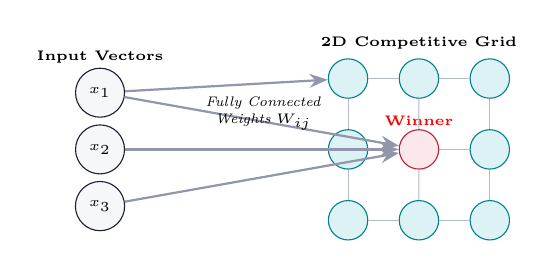
\begin{tikzpicture}[scale=0.9, every node/.style={font=\tiny}]
  % Inputs
  \node[circle, draw=mydark, fill=mygray, minimum size=0.5cm] (x1) at (-2.5, 0.8) {$x_1$};
  \node[circle, draw=mydark, fill=mygray, minimum size=0.5cm] (x2) at (-2.5, 0) {$x_2$};
  \node[circle, draw=mydark, fill=mygray, minimum size=0.5cm] (x3) at (-2.5, -0.8) {$x_3$};
  \node at (-2.5, 1.3) {\textbf{Input Vectors}};

  % 2D Grid
  \node[circle, draw=myteal, fill=hdrteal, minimum size=0.5cm] (g11) at (1, 1) {};
  \node[circle, draw=myteal, fill=hdrteal, minimum size=0.5cm] (g12) at (2, 1) {};
  \node[circle, draw=myteal, fill=hdrteal, minimum size=0.5cm] (g13) at (3, 1) {};
  \node[circle, draw=myteal, fill=hdrteal, minimum size=0.5cm] (g21) at (1, 0) {};
  \node[circle, draw=myteal, fill=hdrred, draw=myred, minimum size=0.5cm] (g22) at (2, 0) {};
  \node[circle, draw=myteal, fill=hdrteal, minimum size=0.5cm] (g23) at (3, 0) {};
  \node[circle, draw=myteal, fill=hdrteal, minimum size=0.5cm] (g31) at (1, -1) {};
  \node[circle, draw=myteal, fill=hdrteal, minimum size=0.5cm] (g32) at (2, -1) {};
  \node[circle, draw=myteal, fill=hdrteal, minimum size=0.5cm] (g33) at (3, -1) {};
  \node at (2, 1.5) {\textbf{2D Competitive Grid}};

  % Winner Highlight
  \node[red, font=\tiny\bfseries] at (2, 0.4) {Winner};

  % Grid Lines representing neighborhood
  \draw[thin, color=mgframe] (g11) -- (g12) -- (g13);
  \draw[thin, color=mgframe] (g21) -- (g22) -- (g23);
  \draw[thin, color=mgframe] (g31) -- (g32) -- (g33);
  \draw[thin, color=mgframe] (g11) -- (g21) -- (g31);
  \draw[thin, color=mgframe] (g12) -- (g22) -- (g32);
  \draw[thin, color=mgframe] (g13) -- (g23) -- (g33);

  % Connections
  \draw[arrow, color=watermark] (x1) -- (g11);
  \draw[arrow, color=watermark] (x1) -- (g22);
  \draw[arrow, color=watermark] (x2) -- (g22);
  \draw[arrow, color=watermark] (x3) -- (g22);
  
  \node at (-0.2, 0.5) [align=center, font=\tiny\itshape] {Fully Connected\\Weights $W_{ij}$};
\end{tikzpicture}
\end{tcolorbox}

\subsection{Kohonen SOM Learning Algorithm}
The training process involves four major steps:
\begin{enumerate}[leftmargin=*, itemsep=3.5pt]
  \item \textbf{Initialization:} Initialize weight vectors $W_j = (w_{j1}, w_{j2}, \ldots, w_{jn})^T$ for each grid node $j$ with small random values. Set parameters: initial learning rate $\alpha_0$ and initial neighborhood radius $\sigma_0$.
  \item \textbf{Similarity Matching (Finding the BMU):} For a given input vector $X = (x_1, x_2, \ldots, x_n)^T$, compute the Euclidean distance to all weight vectors:
    \begin{equation}
      d_j(X) = ||X - W_j|| = \sqrt{\sum_{i=1}^n (x_i - w_{ji})^2}
    \end{equation}
    Identify the winning neuron (Best Matching Unit, BMU) index $c$:
    \begin{equation}
      c = \arg\min_{j} d_j(X)
    \end{equation}
  \item \textbf{Weight Updating:} Update weights of the BMU and all neurons within its neighborhood $h_{cj}(t)$:
    \begin{equation}
      W_j(t+1) = W_j(t) + \alpha(t) h_{cj}(t) [X - W_j(t)]
    \end{equation}
  \item \textbf{Decay Parameters:} Decay the learning rate and the neighborhood size:
    \begin{equation}
      \alpha(t) = \alpha_0 \exp\left(-\frac{t}{\tau_1}\right), \quad \sigma(t) = \sigma_0 \exp\left(-\frac{t}{\tau_2}\right)
    \end{equation}
\end{enumerate}

% ===============================================================================
\section{Learning Vector Quantization (LVQ)}
% ===============================================================================

Learning Vector Quantization (LVQ), introduced by Kohonen, is a supervised competitive learning algorithm used for pattern classification.

\begin{tcolorbox}[defbox, title={LVQ Architecture}]
An \textbf{LVQ network} consists of an input layer and a competitive layer containing codebook vectors (prototype vectors). Each codebook vector is assigned a specific target class.
\end{tcolorbox}

\subsection{LVQ Update Rules}
Let $w_c$ be the codebook vector closest to the input vector $x$ (in terms of Euclidean distance). The weights are adjusted as follows:
\par\noindent
\begin{tcolorbox}[formulabox, title={LVQ Supervised Training updates}]
If the winning codebook vector $w_c$ belongs to the \textbf{correct class} as the input $x$:
\begin{equation}
  w_c(t+1) = w_c(t) + \alpha(t) [x - w_c(t)]
\end{equation}
If the winning codebook vector $w_c$ belongs to an \textbf{incorrect class} relative to input $x$:
\begin{equation}
  w_c(t+1) = w_c(t) - \alpha(t) [x - w_c(t)]
\end{equation}
All other codebook vectors remain unchanged:
\begin{equation}
  w_j(t+1) = w_j(t) \quad \text{for } j \neq c
\end{equation}
\end{tcolorbox}

% ===============================================================================
\section{Counter Propagation Networks (CPN)}
% ===============================================================================

Developed by Robert Hecht-Nielsen in 1987, CPN combines a competitive unsupervised layer (Kohonen SOM) with a self-organizing outstar layer (Grossberg outstar). It acts as a fast lookup table to approximate continuous mathematical functions.

\subsection{CPN Architecture}
CPN contains three layers: Input layer, Kohonen layer (competitive), and Grossberg (Outstar) output layer.

\begin{tcolorbox}[tikzbox, title={Counter Propagation Network (CPN) Layout}]
\centering
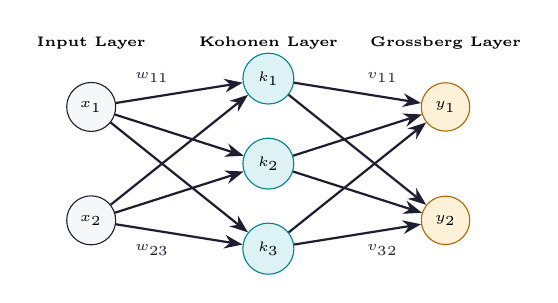
\begin{tikzpicture}[scale=0.9, every node/.style={font=\tiny}]
  % Inputs
  \node[circle, draw=mydark, fill=mygray, minimum size=0.5cm] (x1) at (-2.5, 0.8) {$x_1$};
  \node[circle, draw=mydark, fill=mygray, minimum size=0.5cm] (x2) at (-2.5, -0.8) {$x_2$};
  
  % Kohonen Nodes
  \node[circle, draw=myteal, fill=hdrteal, minimum size=0.5cm] (k1) at (0, 1.2) {$k_1$};
  \node[circle, draw=myteal, fill=hdrteal, minimum size=0.5cm] (k2) at (0, 0) {$k_2$};
  \node[circle, draw=myteal, fill=hdrteal, minimum size=0.5cm] (k3) at (0, -1.2) {$k_3$};
  
  % Grossberg Nodes
  \node[circle, draw=myamber, fill=hdramber, minimum size=0.5cm] (g1) at (2.5, 0.8) {$y_1$};
  \node[circle, draw=myamber, fill=hdramber, minimum size=0.5cm] (g2) at (2.5, -0.8) {$y_2$};

  % Connections: Input to Kohonen (Weights W)
  \draw[arrow] (x1) -- node[midway, above left] {$w_{11}$} (k1);
  \draw[arrow] (x1) -- (k2);
  \draw[arrow] (x1) -- (k3);
  \draw[arrow] (x2) -- (k1);
  \draw[arrow] (x2) -- (k2);
  \draw[arrow] (x2) -- node[midway, below left] {$w_{23}$} (k3);

  % Connections: Kohonen to Grossberg (Weights V)
  \draw[arrow] (k1) -- node[midway, above right] {$v_{11}$} (g1);
  \draw[arrow] (k1) -- (g2);
  \draw[arrow] (k2) -- (g1);
  \draw[arrow] (k2) -- (g2);
  \draw[arrow] (k3) -- (g1);
  \draw[arrow] (k3) -- node[midway, below right] {$v_{32}$} (g2);

  % Layer Labels
  \node at (-2.5, 1.7) {\textbf{Input Layer}};
  \node at (0, 1.7) {\textbf{Kohonen Layer}};
  \node at (2.5, 1.7) {\textbf{Grossberg Layer}};
\end{tikzpicture}
\end{tcolorbox}

\subsection{CPN Training phases}
\begin{enumerate}[leftmargin=*, itemsep=3pt]
  \item \textbf{First Phase (Kohonen Training):} The input vector $X$ is presented. The Kohonen layer acts as a competitive classifier. The winning neuron $c$ is determined, and its weights $W_c$ are updated using standard Kohonen rules.
  \item \textbf{Second Phase (Grossberg Training):} The Kohonen layer outputs a binary vector where only the winning unit has activation $1$, and all others are $0$ ($z_j = \delta_{jc}$). The Grossberg weights $V$ are updated to match the target vector $Y$:
    \begin{equation}
      v_{jk}(t+1) = v_{jk}(t) + \beta [y_k - v_{jk}(t)] z_j
    \end{equation}
    For the winner $c$: $V_c(t+1) = V_c(t) + \beta [Y - V_c(t)]$.
\end{enumerate}

% ===============================================================================
\section{Worked Examples}
% ===============================================================================

\begin{tcolorbox}[examplebox, title={Kohonen SOM Winning Neuron and Weight Update}]
\textbf{Problem:} Given an input vector $X = \begin{bmatrix} 0.8 & 0.6 \end{bmatrix}^T$ and three Kohonen neurons with weight vectors:
\begin{equation*}
  W_1 = \begin{bmatrix} 0.9 & 0.1 \end{bmatrix}^T, \quad W_2 = \begin{bmatrix} 0.7 & 0.5 \end{bmatrix}^T, \quad W_3 = \begin{bmatrix} 0.2 & 0.8 \end{bmatrix}^T
\end{equation*}
\begin{enumerate}[label=(\alph*), leftmargin=*, itemsep=2.5pt]
  \item Identify the winning neuron (BMU) using Euclidean distance.
  \item Update the weight vector of the winning neuron using learning rate $\alpha = 0.5$.
\end{enumerate}
\par\vspace{4pt}\noindent\rule{\linewidth}{0.5pt}\par
\textbf{Solution:}

\textbf{(a) Similarity Matching:}
Compute the squared Euclidean distance $D_j = ||X - W_j||^2$ for each neuron:
\begin{itemize}[leftmargin=*, itemsep=2pt]
  \item For $W_1$:
    \begin{equation*}
      D_1 = (0.8 - 0.9)^2 + (0.6 - 0.1)^2 = (-0.1)^2 + (0.5)^2 = 0.01 + 0.25 = 0.26
    \end{equation*}
  \item For $W_2$:
    \begin{equation*}
      D_2 = (0.8 - 0.7)^2 + (0.6 - 0.5)^2 = (0.1)^2 + (0.1)^2 = 0.01 + 0.01 = 0.02
    \end{equation*}
  \item For $W_3$:
    \begin{equation*}
      D_3 = (0.8 - 0.2)^2 + (0.6 - 0.8)^2 = (0.6)^2 + (-0.2)^2 = 0.36 + 0.04 = 0.40
    \end{equation*}
\end{itemize}
Since $D_2 = 0.02$ is the minimum, \textbf{Neuron 2 ($W_2$)} is the winning neuron (BMU).

\par\vspace{4pt}
\textbf{(b) Weight Update:}
Update the weights of the winning neuron $W_2$:
\begin{align*}
  W_2(new) &= W_2(old) + \alpha [X - W_2(old)] \\
  &= \begin{bmatrix} 0.7 \\ 0.5 \end{bmatrix} + 0.5 \left( \begin{bmatrix} 0.8 \\ 0.6 \end{bmatrix} - \begin{bmatrix} 0.7 \\ 0.5 \end{bmatrix} \right) \\
  &= \begin{bmatrix} 0.7 \\ 0.5 \end{bmatrix} + 0.5 \begin{bmatrix} 0.1 \\ 0.1 \end{bmatrix} = \begin{bmatrix} 0.7 \\ 0.5 \end{bmatrix} + \begin{bmatrix} 0.05 \\ 0.05 \end{bmatrix} = \begin{bmatrix} 0.75 \\ 0.55 \end{bmatrix}
\end{align*}
The updated weight vector is $W_2 = \begin{bmatrix} 0.75 & 0.55 \end{bmatrix}^T$.
\end{tcolorbox}

\begin{tcolorbox}[examplebox, title={LVQ Classifier Updates}]
\textbf{Problem:} Given an input vector $x = \begin{bmatrix} 0.1 & 0.9 \end{bmatrix}$ belonging to Class 1, and the closest codebook vector $w_c = \begin{bmatrix} 0.2 & 0.7 \end{bmatrix}$. 
Calculate the updated codebook vector for:
\begin{enumerate}[label=(\alph*), leftmargin=*]
  \item Class of $w_c$ is Class 1 (correct class)
  \item Class of $w_c$ is Class 2 (incorrect class)
\end{enumerate}
Assume learning rate $\alpha = 0.2$.
\par\vspace{4pt}\noindent\rule{\linewidth}{0.5pt}\par
\textbf{Solution:}

\textbf{(a) Correct Class Update (Push towards input):}
\begin{align*}
  w_c(new) &= w_c(old) + \alpha [x - w_c(old)] \\
  &= \begin{bmatrix} 0.2 \\ 0.7 \end{bmatrix} + 0.2 \left( \begin{bmatrix} 0.1 \\ 0.9 \end{bmatrix} - \begin{bmatrix} 0.2 \\ 0.7 \end{bmatrix} \right) \\
  &= \begin{bmatrix} 0.2 \\ 0.7 \end{bmatrix} + 0.2 \begin{bmatrix} -0.1 \\ 0.2 \end{bmatrix} = \begin{bmatrix} 0.2 - 0.02 \\ 0.7 + 0.04 \end{bmatrix} = \begin{bmatrix} 0.18 \\ 0.74 \end{bmatrix}
\end{align*}

\textbf{(b) Incorrect Class Update (Pull away from input):}
\begin{align*}
  w_c(new) &= w_c(old) - \alpha [x - w_c(old)] \\
  &= \begin{bmatrix} 0.2 \\ 0.7 \end{bmatrix} - 0.2 \left( \begin{bmatrix} 0.1 \\ 0.9 \end{bmatrix} - \begin{bmatrix} 0.2 \\ 0.7 \end{bmatrix} \right) \\
  &= \begin{bmatrix} 0.2 \\ 0.7 \end{bmatrix} - 0.2 \begin{bmatrix} -0.1 \\ 0.2 \end{bmatrix} = \begin{bmatrix} 0.2 + 0.02 \\ 0.7 - 0.04 \end{bmatrix} = \begin{bmatrix} 0.22 \\ 0.66 \end{bmatrix}
\end{align*}
\end{tcolorbox}

\newpage

% ===============================================================================
% MANDATORY QUICK REVISION PAGE
% ===============================================================================
\begin{center}
  {\large\bfseries\color{myred} Quick Revision --- Module II}\\[3pt]
  {\small\color{mydark} Competitive Neural Networks $|$ PE-EC702C}
\end{center}
\noindent{\color{myred}\rule{\linewidth}{1.2pt}}
\vspace{4pt}

\begin{tcolorbox}[formulabox, title={\textbf{Key Formulas at a Glance}}]
\renewcommand{\arraystretch}{1.3}
\begin{tabularx}{\linewidth}{B{5.0cm} X}Euclidean Distance in SOM & $d_j(X) = \sqrt{\sum_{i=1}^n (x_i - w_{ji})^2}$ \\
Winning Neuron (BMU) Index & $c = \arg\min_j d_j(X)$ \\
Kohonen Weight Update & $W_j(t+1) = W_j(t) + \alpha(t) h_{cj}(t) [X - W_j(t)]$ \\
LVQ Correct Update & $w_c(t+1) = w_c(t) + \alpha(t) [x - w_c(t)]$ \\
LVQ Incorrect Update & $w_c(t+1) = w_c(t) - \alpha(t) [x - w_c(t)]$ \\
Grossberg outstar Update & $V_c(t+1) = V_c(t) + \beta [Y - V_c(t)]$
\end{tabularx}
\end{tcolorbox}

\begin{tcolorbox}[defbox, title={\textbf{One-Line Definitions}}]
\begin{itemize}[leftmargin=*, itemsep=2.5pt, topsep=0pt]
  \item \textbf{Kohonen SOM:} An unsupervised clustering network that creates a topology-preserving mapping of high-dimensional input features.
  \item \textbf{Best Matching Unit (BMU):} The neuron in a competitive layer whose weight vector is closest to the current input vector.
  \item \textbf{LVQ:} A supervised competitive network that uses prototype vectors to map inputs to specific classification boundaries.
  \item \textbf{CPN:} A hybrid network that maps input patterns to target vectors rapidly by combining a Kohonen layer with a Grossberg layer.
  \item \textbf{Grossberg Outstar:} A learning unit designed to output a specific analog target pattern when triggered by a Kohonen node.
\end{itemize}
\end{tcolorbox}

\begin{tcolorbox}[exambox, title={\textbf{Frequently Asked / Viva Questions}}]
\begin{enumerate}[leftmargin=*, itemsep=3.5pt, label=\arabic*.]
  \item \Q{What is the primary difference between Perceptron learning and Kohonen learning?} Perceptron learning is supervised and minimizes output error feedback. Kohonen learning is unsupervised and uses similarity metrics to cluster features.
  \item \Q{How does the neighborhood function $h_{cj}(t)$ change during SOM training?} It starts wide to organize the global structure of the map, and then shrinks exponentially over time to allow fine-tuning of local weights.
  \item \Q{Why is LVQ considered a supervised learning algorithm while SOM is unsupervised?} SOM groups data based solely on input similarities without class labels. LVQ adjusts its codebook vectors based on class labels to optimize classification boundaries.
  \item \Q{Explain the role of Grossberg outstar layer in Counter Propagation Networks.} The Kohonen layer maps inputs to a single active winning unit. The Grossberg layer acts as a lookup table, outputting a stored target vector associated with that unit.
  \item \Q{What is the significance of the vigilance parameter in competitive networks?} It controls the sensitivity of node matching. In networks like ART, it determines if a new cluster must be created or if the input fits an existing cluster.
  \item \Q{Why does CPN train faster than Backpropagation networks?} CPN updates only the winning Kohonen neuron and the corresponding Grossberg weights, avoiding expensive error propagation across multiple layers.
  \item \Q{What is the purpose of lateral inhibition in competitive networks?} It allows active neurons to suppress the activation of neighboring competitive neurons, ensuring that only one winning neuron (the BMU) remains active.
  \item \Q{How does LVQ-2 differ from standard LVQ-1?} LVQ-1 updates only the single closest codebook vector. LVQ-2 updates the two closest vectors simultaneously if the input falls near the decision boundary.
  \item \Q{What is meant by a topology-preserving mapping in SOM?} It means that input vectors that are close in the high-dimensional feature space are mapped to neurons that are close to each other on the 2D output grid.
  \item \Q{What is the codebook vector in Learning Vector Quantization?} It is a prototype vector representing a class cluster center in the input space.
\end{enumerate}
\end{tcolorbox}

\begin{tcolorbox}[tikzbox, title={Comparison of Competitive Networks}]
\centering
{\renewcommand{\arraystretch}{1.55}%
\begin{tabularx}{\linewidth}{|>{\bfseries}B{3.2cm}|Y|Y|Y|}
\hline
Attribute & Kohonen SOM & LVQ & CPN \\
\hline
Learning Type & Unsupervised & Supervised & Hybrid (Supervised + Unsupervised) \\
\hline
Primary Application & Dimensionality reduction & Pattern classification & Function approximation \\
\hline
Output Layer Grid & 1D or 2D grid structure & 1D array of vectors & 1D array of output nodes \\
\hline
Weight Updates & Updates winner + neighbors & Updates winner only & Updates winner only \\
\hline
\end{tabularx}}
\end{tcolorbox}


% -- Module 3 -----------------------------------------------------------------
\modulestart{3}{Backpropagation Neural Networks (BPNN)}

\section{Backpropagation Neural Networks (BPNN)}
% ===============================================================================

The Backpropagation algorithm is the standard method for training Multi-Layer Perceptrons (MLPs). It is a supervised learning method based on the generalized delta rule (gradient descent on error space).

\begin{tcolorbox}[defbox, title={Multi-Layer Perceptron (MLP)}]
A \textbf{Multi-Layer Perceptron (MLP)} is a feedforward artificial neural network topology consisting of an input layer, one or more hidden layers, and an output layer of non-linear processing units.
\end{tcolorbox}

\begin{tcolorbox}[tikzbox, title={Multi-Layer Perceptron Feedforward Architecture}]
\centering
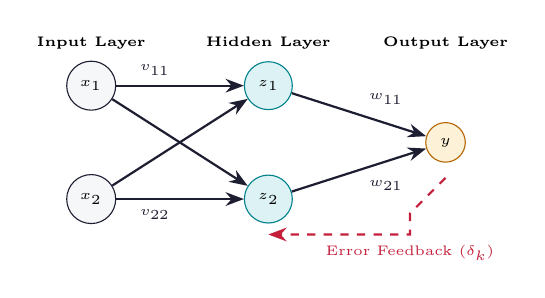
\begin{tikzpicture}[scale=0.9, every node/.style={font=\tiny}]
  % Input Layer
  \node[circle, draw=mydark, fill=mygray, minimum size=0.5cm] (x1) at (-2.5, 0.8) {$x_1$};
  \node[circle, draw=mydark, fill=mygray, minimum size=0.5cm] (x2) at (-2.5, -0.8) {$x_2$};
  \node at (-2.5, 1.4) {\textbf{Input Layer}};

  % Hidden Layer
  \node[circle, draw=myteal, fill=hdrteal, minimum size=0.5cm] (z1) at (0, 0.8) {$z_1$};
  \node[circle, draw=myteal, fill=hdrteal, minimum size=0.5cm] (z2) at (0, -0.8) {$z_2$};
  \node at (0, 1.4) {\textbf{Hidden Layer}};

  % Output Layer
  \node[circle, draw=myamber, fill=hdramber, minimum size=0.5cm] (y) at (2.5, 0) {$y$};
  \node at (2.5, 1.4) {\textbf{Output Layer}};

  % Connections: Input to Hidden
  \draw[arrow] (x1) -- node[midway, above left] {$v_{11}$} (z1);
  \draw[arrow] (x1) -- (z2);
  \draw[arrow] (x2) -- (z1);
  \draw[arrow] (x2) -- node[midway, below left] {$v_{22}$} (z2);

  % Connections: Hidden to Output
  \draw[arrow] (z1) -- node[midway, above right] {$w_{11}$} (y);
  \draw[arrow] (z2) -- node[midway, below right] {$w_{21}$} (y);
  
  % Error propagation path
  \draw[dashed, arrow, color=myred] (2.5, -0.5) -- +(-0.5, -0.5) |- (0, -1.3) node[midway, below] {Error Feedback ($\delta_k$)};
\end{tikzpicture}
\end{tcolorbox}

\subsection{Derivation of the Backpropagation Learning Rules}
Let $E$ be the total sum-of-squares error over the output units:
\begin{equation}
  E = \frac{1}{2} \sum_{k} (t_k - y_k)^2
\end{equation}
where $t_k$ is the target output and $y_k$ is the computed activation of output unit $k$.
The activation function used is the binary sigmoid:
\begin{equation}
  y_k = f(net_k) = \frac{1}{1 + e^{-net_k}} \quad \rightarrow \quad f'(net_k) = y_k(1 - y_k)
\end{equation}
where $net_k = \sum_{j} w_{kj} z_j + b_k$ ($z_j$ is the activation of hidden node $j$).

\par\noindent
Using gradient descent, the weight changes are proportional to the negative gradient of error:
\begin{equation}
  \Delta w_{kj} = -\eta \frac{\partial E}{\partial w_{kj}}
\end{equation}
By applying the chain rule of calculus:
\begin{equation}
  \frac{\partial E}{\partial w_{kj}} = \frac{\partial E}{\partial y_k} \cdot \frac{\partial y_k}{\partial net_k} \cdot \frac{\partial net_k}{\partial w_{kj}}
\end{equation}
Evaluating each derivative:
\begin{equation*}
  \frac{\partial E}{\partial y_k} = -(t_k - y_k), \quad \frac{\partial y_k}{\partial net_k} = f'(net_k) = y_k(1 - y_k), \quad \frac{\partial net_k}{\partial w_{kj}} = z_j
\end{equation*}
Substituting these terms back:
\begin{equation}
  \frac{\partial E}{\partial w_{kj}} = -(t_k - y_k) f'(net_k) z_j
\end{equation}
Defining the error term (delta) for output unit $k$ as $\delta_k = (t_k - y_k) f'(net_k)$:
\begin{equation}
  \Delta w_{kj} = \eta \delta_k z_j
\end{equation}

\par\noindent
For input-to-hidden weights $v_{ji}$ connecting input $i$ to hidden unit $j$:
\begin{equation}
  \Delta v_{ji} = -\eta \frac{\partial E}{\partial v_{ji}} = -\eta \frac{\partial E}{\partial z_j} \cdot \frac{\partial z_j}{\partial net_j} \cdot \frac{\partial net_j}{\partial v_{ji}}
\end{equation}
where $z_j = f(net_j)$ and $net_j = \sum_i v_{ji} x_i + b_j$.
The error gradient relative to hidden activation $z_j$ accumulates from all output nodes:
\begin{equation*}
  \frac{\partial E}{\partial z_j} = \sum_k \frac{\partial E}{\partial net_k} \cdot \frac{\partial net_k}{\partial z_j} = \sum_k (-\delta_k) w_{kj}
\end{equation*}
Applying the other terms:
\begin{equation*}
  \frac{\partial z_j}{\partial net_j} = f'(net_j) = z_j(1 - z_j), \quad \frac{\partial net_j}{\partial v_{ji}} = x_i
\end{equation*}
Defining the error term (delta) for hidden unit $j$ as $\delta_j = f'(net_j) \sum_k \delta_k w_{kj}$:
\begin{equation}
  \Delta v_{ji} = \eta \delta_j x_i
\end{equation}

% ===============================================================================
\section{Adaptive Resonance Theory (ART)}
% ===============================================================================

Developed by Stephen Grossberg and Gail Carpenter (1987), ART is designed to solve the stability-plasticity dilemma in unsupervised neural networks.

\begin{tcolorbox}[defbox, title={Stability-Plasticity Dilemma}]
\textbf{Stability-Plasticity Dilemma:} The challenge of designing a learning system that remains adaptive to new patterns (plasticity) while preventing new learning from washing out previously acquired knowledge (stability).
\end{tcolorbox}

\subsection{ART1 vs. ART2}
\begin{itemize}[leftmargin=*, itemsep=3pt]
  \item \textbf{ART1:} Designed to process binary input vectors ($\{0, 1\}$).
  \item \textbf{ART2:} Designed to process continuous (analog) input vectors.
\end{itemize}

\subsection{ART1 Architecture and Operation}
ART1 consists of two subsystems: the Attentional Subsystem and the Orienting Subsystem.

\begin{tcolorbox}[tikzbox, title={ART1 Network Architecture}]
\centering
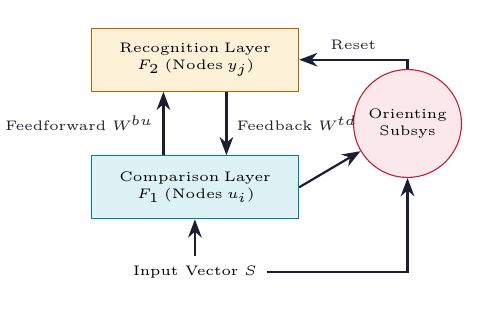
\begin{tikzpicture}[scale=0.9, every node/.style={font=\tiny}]
  % Comparison Layer (F1)
  \node[rectangle, draw=myteal, fill=hdrteal, text width=2.4cm, align=center, minimum height=0.8cm] (f1) at (0, 0) {Comparison Layer\\$F_1$ (Nodes $u_i$)};
  
  % Recognition Layer (F2)
  \node[rectangle, draw=myamber, fill=hdramber, text width=2.4cm, align=center, minimum height=0.8cm] (f2) at (0, 1.8) {Recognition Layer\\$F_2$ (Nodes $y_j$)};

  % Orienting Subsystem (Reset)
  \node[circle, draw=myred, fill=hdrred, minimum size=0.8cm, align=center] (orient) at (3.0, 0.9) {Orienting\\Subsys};

  % Feedback and Feedforward arrows
  \draw[arrow, transform canvas={xshift=-0.4cm}] (f1.north) -- node[midway, left] {Feedforward $W^{bu}$} (f2.south);
  \draw[arrow, transform canvas={xshift=0.4cm}] (f2.south) -- node[midway, right] {Feedback $W^{td}$} (f1.north);

  % Inputs
  \node (in) at (0, -1.2) {Input Vector $S$};
  \draw[arrow] (in) -- (f1);

  % Vigilance comparison
  \draw[arrow] (in.east) -| (orient);
  \draw[arrow] (f1.east) -- (orient);
  \draw[arrow] (orient.north) |- (f2.east) node[near end, above] {Reset};
\end{tikzpicture}
\end{tcolorbox}

\par\noindent
\textbf{Working Mechanism:}
\begin{enumerate}[leftmargin=*, itemsep=2.5pt]
  \item \textbf{Input presentation:} Input $S$ is sent to the $F_1$ layer.
  \item \textbf{Feedforward activation:} $F_1$ transmits the pattern to the $F_2$ layer. The $F_2$ layer is a competitive layer where the node with the highest net input wins (winner-take-all).
  \item \textbf{Feedback Template matching:} The winning $F_2$ neuron projects its prototype vector (template) back down to $F_1$.
  \item \textbf{Vigilance Test:} The orienting subsystem calculates the ratio of match:
    \begin{equation}
      \frac{|S \cap X|}{|S|}
    \end{equation}
    where $X$ is the activation of the $F_1$ layer.
    \begin{itemize}[leftmargin=1.5em, itemsep=1.5pt]
      \item If ratio $\ge \rho$ (vigilance parameter), \textbf{resonance} occurs. The network accepts the match and updates the winning neuron's weights.
      \item If ratio $< \rho$, the orienting subsystem sends a \textbf{reset signal} to temporarily disable the winning $F_2$ node. The search process repeats for other $F_2$ nodes. If no match is found, a new category node is initialized.
    \end{itemize}
\end{enumerate}

% ===============================================================================
\section{Boltzmann Machine Learning}
% ===============================================================================

The Boltzmann Machine is a recurrent, symmetrically connected network consisting of stochastic binary units (visible and hidden) that operate under statistical thermodynamics principles.

\begin{tcolorbox}[formulabox, title={Boltzmann Energy \& Transition Rules}]
The total energy $E$ of a Boltzmann state configuration is defined as:
\begin{equation}
  E = -\sum_{i < j} w_{ij} s_i s_j - \sum_{i} \theta_i s_i
\end{equation}
where $w_{ij}$ is the connection weight, $s_i \in \{0, 1\}$ is the state of unit $i$, and $\theta_i$ is the threshold bias.
\par\noindent
The probability that unit $i$ transitions to state $s_i = 1$ is given by the sigmoid-like logistic function:
\begin{equation}
  P(s_i = 1) = \frac{1}{1 + e^{-\Delta E_i / T}}
\end{equation}
where $\Delta E_i = \sum_j w_{ij} s_j + \theta_i$ is the energy difference and $T$ is the temperature parameter.
\end{tcolorbox}

\subsection{Boltzmann Learning Rule}
Boltzmann training occurs in two distinct phases:
\begin{enumerate}[leftmargin=*, itemsep=3.5pt]
  \item \textbf{Positive (Clamped) Phase:} The visible units are clamped to target training patterns. The network is allowed to reach thermal equilibrium, and the correlation probabilities $p_{ij}^+$ that units $i$ and $j$ are active simultaneously are measured.
  \item \textbf{Negative (Free-Running) Phase:} No units are clamped. The network runs freely to reach thermal equilibrium, and the free probabilities $p_{ij}^-$ are measured.
  \item \textbf{Weight Update:} Weights are updated to minimize Kullback-Leibler divergence:
    \begin{equation}
      \Delta w_{ij} = \eta (p_{ij}^+ - p_{ij}^-)
    \end{equation}
\end{enumerate}

% ===============================================================================
\section{Worked Examples}
% ===============================================================================

\begin{tcolorbox}[examplebox, title={Backpropagation Step-by-Step Numerical}]
\textbf{Problem:} Consider a simplified neural network containing 1 input node ($x$), 1 hidden node ($z$), and 1 output node ($y$). The transfer function is the binary sigmoid: $f(net) = 1/(1 + e^{-net})$. 
\par
Given: Input $x = 1.0$, target $t = 0.9$, learning rate $\eta = 0.5$.
Initial weights and biases:
\begin{itemize}[leftmargin=*, itemsep=2pt]
  \item Input-to-hidden weight $v = 0.5$, bias $b_1 = 0.2$
  \item Hidden-to-output weight $w = 0.8$, bias $b_2 = 0.1$
\end{itemize}
Calculate the updated weights $w$ and $v$ after a single backpropagation epoch.
\par\vspace{4pt}\noindent\rule{\linewidth}{0.5pt}\par
\textbf{Solution:}

\textbf{1. Forward Pass:}
\begin{itemize}[leftmargin=*, itemsep=2.5pt]
  \item \textbf{Hidden Node $z$:}
    \begin{align*}
      net_z &= v \cdot x + b_1 = 0.5(1.0) + 0.2 = 0.7 \\
      z &= f(net_z) = \frac{1}{1 + e^{-0.7}} \approx 0.668
    \end{align*}
  \item \textbf{Output Node $y$:}
    \begin{align*}
      net_y &= w \cdot z + b_2 = 0.8(0.668) + 0.1 \approx 0.634 \\
      y &= f(net_y) = \frac{1}{1 + e^{-0.634}} \approx 0.653
    \end{align*}
\end{itemize}

\par\vspace{4pt}
\textbf{2. Backward Pass (Error Propagation):}
\begin{itemize}[leftmargin=*, itemsep=2.5pt]
  \item \textbf{Output Delta ($\delta_y$):}
    \begin{align*}
      \delta_y &= (t - y) y (1 - y) \\
      &= (0.9 - 0.653) \cdot 0.653 \cdot (1 - 0.653) \\
      &= 0.247 \cdot 0.653 \cdot 0.347 \approx 0.0560
    \end{align*}
  \item \textbf{Hidden Delta ($\delta_z$):}
    \begin{align*}
      \delta_z &= \delta_y \cdot w \cdot z(1 - z) \\
      &= 0.0560 \cdot 0.8 \cdot 0.668 \cdot (1 - 0.668) \\
      &= 0.0448 \cdot 0.668 \cdot 0.332 \approx 0.00993
    \end{align*}
\end{itemize}

\par\vspace{4pt}
\textbf{3. Weight Updates:}
\begin{itemize}[leftmargin=*, itemsep=2.5pt]
  \item \textbf{Hidden-to-Output Weight ($w$):}
    \begin{align*}
      \Delta w &= \eta \cdot \delta_y \cdot z = 0.5 \cdot 0.0560 \cdot 0.668 \approx 0.0187 \\
      w(new) &= 0.8 + 0.0187 = 0.8187
    \end{align*}
  \item \textbf{Input-to-Hidden Weight ($v$):}
    \begin{align*}
      \Delta v &= \eta \cdot \delta_z \cdot x = 0.5 \cdot 0.00993 \cdot 1.0 \approx 0.00497 \\
      v(new) &= 0.5 + 0.00497 = 0.50497
    \end{align*}
\end{itemize}
The updated weights are $w \approx 0.8187$ and $v \approx 0.5050$.
\end{tcolorbox}

\newpage

% ===============================================================================
% MANDATORY QUICK REVISION PAGE
% ===============================================================================
\begin{center}
  {\large\bfseries\color{myred} Quick Revision --- Module III}\\[3pt]
  {\small\color{mydark} Adaptive Resonance \& Backpropagation $|$ PE-EC702C}
\end{center}
\noindent{\color{myred}\rule{\linewidth}{1.2pt}}
\vspace{4pt}

\begin{tcolorbox}[formulabox, title={\textbf{Key Formulas at a Glance}}]
\renewcommand{\arraystretch}{1.3}
\begin{tabularx}{\linewidth}{B{5.0cm} X}Total Output Error & $E = \frac{1}{2} \sum_{k} (t_k - y_k)^2$ \\
Output Layer Delta ($\delta_k$) & $\delta_k = (t_k - y_k) y_k (1 - y_k) \quad \text{(for sigmoid)}$ \\
Hidden Layer Delta ($\delta_j$) & $\delta_j = z_j(1 - z_j) \sum_{k} \delta_k w_{kj} \quad \text{(for sigmoid)}$ \\
BPNN Weight Updates & $\Delta w_{kj} = \eta \delta_k z_j, \quad \Delta v_{ji} = \eta \delta_j x_i$ \\
ART1 Vigilance Ratio & Match $= \frac{|S \cap X|}{|S|} \ge \rho \quad \text{(where } \rho \in [0, 1]\text{)}$ \\
Boltzmann Energy Configuration & $E = -\sum_{i < j} w_{ij} s_i s_j - \sum_i \theta_i s_i$
\end{tabularx}
\end{tcolorbox}

\begin{tcolorbox}[defbox, title={\textbf{One-Line Definitions}}]
\begin{itemize}[leftmargin=*, itemsep=2.5pt, topsep=0pt]
  \item \textbf{Backpropagation:} A supervised gradient-descent algorithm that updates network weights to minimize the sum of squared errors.
  \item \textbf{Stability-Plasticity Dilemma:} The goal of learning new input patterns without overwriting previously learned representations.
  \item \textbf{Vigilance Parameter ($\rho$):} The threshold parameter in ART that determines how closely an input must match a category template.
  \item \textbf{Resonance:} The state in ART where an input matches a template well enough to initiate weight tuning.
  \item \textbf{Boltzmann Machine:} A recurrent stochastic neural network that uses simulated annealing to escape local energy minima.
\end{itemize}
\end{tcolorbox}

\begin{tcolorbox}[exambox, title={\textbf{Frequently Asked / Viva Questions}}]
\begin{enumerate}[leftmargin=*, itemsep=3.5pt, label=\arabic*.]
  \item \Q{Why is Backpropagation referred to as a "supervised" learning algorithm?} Because weight adjustments are calculated using the difference (error) between the network's computed output and the target (label) vector.
  \item \Q{State the purpose of the activation function's derivative $f'(net)$ in backpropagation.} It scales the weight update based on the slope of the activation curve. In flat regions (near $0$ or $1$ for sigmoids), updates are very small, preventing oscillations.
  \item \Q{What is the effect of setting a high vigilance parameter ($\rho$) in ART1?} A high vigilance value (e.g. $\rho = 0.95$) requires highly precise matches, leading the network to create many narrow, fine-grained categories.
  \item \Q{What is the effect of setting a low vigilance parameter ($\rho$) in ART1?} A low vigilance value (e.g. $\rho = 0.3$) allows loose matching, causing the network to group highly different inputs into a few broad, coarse categories.
  \item \Q{How does Boltzmann learning utilize the positive and negative phases?} The positive phase clamps inputs to capture target correlations ($p_{ij}^+$), while the negative phase runs freely to capture network-generated correlations ($p_{ij}^-$).
  \item \Q{Why does backpropagation sometimes get stuck in local minima?} Because gradient descent follows local gradients on the error surface. If it enters a local valley (minimum) that is not the absolute lowest point (global minimum), it cannot escape.
  \item \Q{What is the function of the orienting subsystem in ART1?} It acts as a controller that compares the input match ratio with the vigilance parameter $\rho$. If it is too low, it issues a reset signal to disable the winning category node.
  \item \Q{Define the term "Simulated Annealing" in Boltzmann machines.} The process of starting at a high temperature $T$ to allow stochastic state jumps (escaping local minima), and slowly cooling down to settle in the global minimum state.
  \item \Q{What is the difference between feedforward and feedback networks in terms of stability?} Feedforward networks compute outputs instantaneously and are always stable. Feedback networks have recurrent loop dynamics and can oscillate or require iterative convergence to reach stability.
  \item \Q{Why is $\frac{1}{2}$ added in the error formulation $E = \frac{1}{2}\sum(t-y)^2$?} It is a mathematical convenience that cancels out the coefficient $2$ when taking the derivative $\frac{\partial E}{\partial y} = -(t-y)$ during gradient calculations.
\end{enumerate}
\tcbset{colbacktitle=myteal, coltitle=white}
\end{tcolorbox}

\begin{tcolorbox}[tikzbox, title={Comparison of Adaptive Architectures}]
\centering
{\renewcommand{\arraystretch}{1.55}%
\begin{tabularx}{\linewidth}{|>{\bfseries}B{3.2cm}|Y|Y|Y|}
\hline
Attribute & Backpropagation BPNN & ART1 & Boltzmann Machine \\
\hline
Learning Type & Supervised & Unsupervised & Supervised / Unsupervised \\
\hline
Connections & Feedforward only & Bidirectional (top-down/bottom-up) & Symmetric recurrent loops \\
\hline
Neuron States & Analog / Continuous & Binary $\{0, 1\}$ & Stochastic Binary $\{0, 1\}$ \\
\hline
Page Resolution & Fixed classes & Dynamic category creation & Probability distribution fitting \\
\hline
\end{tabularx}}
\tcbset{colbacktitle=myteal, coltitle=white}
\end{tcolorbox}


% -- Module 4 -----------------------------------------------------------------
\modulestart{4}{Classical (Crisp) Sets vs. Fuzzy Sets}

\section{Classical (Crisp) Sets vs. Fuzzy Sets}
% ===============================================================================

Classical set theory is based on binary logic (true/false, black/white), whereas fuzzy set theory allows for gradual transitions and degrees of membership.

\begin{tcolorbox}[defbox, title={Fuzzy Set}]
A \textbf{Fuzzy Set} $A$ in a universe of discourse $U$ is defined by a membership function $\mu_A(x)$ that maps each element $x \in U$ to a continuous value in the interval $[0, 1]$.
\begin{equation}
  A = \left\{ \left( x, \mu_A(x) \right) \mid x \in U \right\}
\end{equation}
\end{tcolorbox}

\subsection{Standard Fuzzy Operations}
Let $A$ and $B$ be two fuzzy sets with membership functions $\mu_A(x)$ and $\mu_B(x)$ respectively:
\begin{itemize}[leftmargin=*, itemsep=3.5pt]
  \item \textbf{Union (OR / Standard Max):}
    \begin{equation}
      \mu_{A \cup B}(x) = \max\left( \mu_A(x), \mu_B(x) \right) = \mu_A(x) \lor \mu_B(x)
    \end{equation}
  \item \textbf{Intersection (AND / Standard Min):}
    \begin{equation}
      \mu_{A \cap B}(x) = \min\left( \mu_A(x), \mu_B(x) \right) = \mu_A(x) \land \mu_B(x)
    \end{equation}
  \item \textbf{Complement (NOT):}
    \begin{equation}
      \mu_{\bar{A}}(x) = 1 - \mu_A(x)
    \end{equation}
  \item \textbf{Algebraic Product (Dot):} $\mu_{A \cdot B}(x) = \mu_A(x) \cdot \mu_B(x)$
  \item \textbf{Algebraic Sum (Probabilistic sum):} $\mu_{A \hat{+} B}(x) = \mu_A(x) + \mu_B(x) - \mu_A(x)\mu_B(x)$
\end{itemize}

% ===============================================================================
\section{Fuzzy Relations and Composition}
% ===============================================================================

Fuzzy relations map elements from universe $X$ to universe $Y$ with a membership value in $[0, 1]$.

\begin{tcolorbox}[formulabox, title={Fuzzy Compositions}]
Let $R$ be a fuzzy relation from $X$ to $Y$, and $S$ be a fuzzy relation from $Y$ to $Z$.
\par\vspace{4pt}
\textbf{1. Max-Min Composition ($T = R \circ S$):}
\begin{equation}
  \mu_T(x, z) = \max_{y \in Y} \left\{ \min\left( \mu_R(x,y), \mu_S(y,z) \right) \right\}
\end{equation}
\textbf{2. Max-Product Composition ($T = R \bullet S$):}
\begin{equation}
  \mu_T(x, z) = \max_{y \in Y} \left\{ \mu_R(x,y) \cdot \mu_S(y,z) \right\}
\end{equation}
\end{tcolorbox}

\subsection{Tolerance and Equivalence Relations}
Fuzzy relations can possess algebraic properties similar to classical relations:
\begin{itemize}[leftmargin=*, itemsep=3.5pt]
  \item \textbf{Reflexivity:} A relation $R$ on set $X$ is reflexive if the membership of any element paired with itself is 1:
    \begin{equation}
      \mu_R(x, x) = 1 \quad \forall x \in X
    \end{equation}
  \item \textbf{Symmetry:} A relation $R$ is symmetric if order of elements does not affect membership:
    \begin{equation}
      \mu_R(x, y) = \mu_R(y, x) \quad \forall x, y \in X
    \end{equation}
  \item \textbf{Transitivity (Max-Min Transitivity):} A relation $R$ is Max-Min transitive if:
    \begin{equation}
      R \circ R \subseteq R \quad \implies \quad \mu_R(x, z) \ge \max_{y \in X} \left\{ \min\left( \mu_R(x, y), \mu_R(y, z) \right) \right\} \quad \forall x, z \in X
    \end{equation}
\end{itemize}

Based on these properties, we define two special fuzzy relations:
\begin{enumerate}[leftmargin=*, itemsep=3.5pt]
  \item \textbf{Tolerance Relation (Compatibility Relation):} A fuzzy relation that is \textbf{reflexive} and \textbf{symmetric}, but not necessarily transitive. It measures the degree of similarity or compatibility between elements.
  \item \textbf{Equivalence Relation (Similarity Relation):} A fuzzy relation that is \textbf{reflexive}, \textbf{symmetric}, and \textbf{Max-Min transitive}. It generalizes the classical equivalence relation to group elements into fuzzy equivalence classes.
\end{enumerate}

% ===============================================================================
\section{Membership Functions and Standard Forms}
% ===============================================================================

\subsection{Key Geometric Features}
\begin{itemize}[leftmargin=*, itemsep=3pt]
  \item \textbf{Support:} The crisp set containing all elements with non-zero membership: $\{x \in U \mid \mu_A(x) > 0\}$.
  \item \textbf{Core:} The crisp set containing all elements with full membership: $\{x \in U \mid \mu_A(x) = 1\}$.
  \item \textbf{Boundary:} The region with $0 < \mu_A(x) < 1$.
  \item \textbf{Crossover Points:} The elements where membership is exactly $0.5$: $\{x \in U \mid \mu_A(x) = 0.5\}$.
\end{itemize}

\subsection{Standard Shapes}
Standard shapes are used to represent categories like "Warm Temperature" or "High Voltage":

\begin{tcolorbox}[tikzbox, title={Standard Membership Function Shapes}]
\centering
\begin{minipage}{0.48\textwidth}
  \centering
  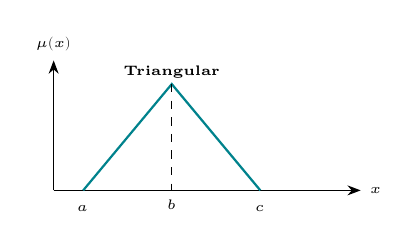
\begin{tikzpicture}[scale=0.75]
    % Axes
    \draw[-Stealth] (0,0) -- (5.2,0) node[right] {\tiny $x$};
    \draw[-Stealth] (0,0) -- (0,2.2) node[above] {\tiny $\mu(x)$};
    % Triangular
    \draw[thick, color=myteal] (0.5,0) -- (2.0,1.8) -- (3.5,0);
    \draw[dashed] (2.0,1.8) -- (2.0,0) node[below] {\tiny $b$};
    \node at (0.5, -0.3) {\tiny $a$};
    \node at (3.5, -0.3) {\tiny $c$};
    \node at (2.0, 2.0) {\textbf{\tiny Triangular}};
  \end{tikzpicture}
\end{minipage}
\hfill
\begin{minipage}{0.48\textwidth}
  \centering
  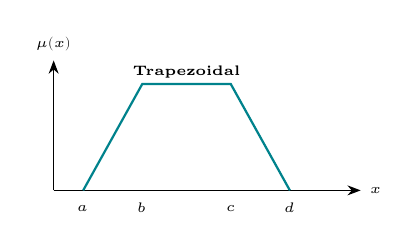
\begin{tikzpicture}[scale=0.75]
    % Axes
    \draw[-Stealth] (0,0) -- (5.2,0) node[right] {\tiny $x$};
    \draw[-Stealth] (0,0) -- (0,2.2) node[above] {\tiny $\mu(x)$};
    % Trapezoidal
    \draw[thick, color=myteal] (0.5,0) -- (1.5,1.8) -- (3.0,1.8) -- (4.0,0);
    \node at (0.5, -0.3) {\tiny $a$};
    \node at (1.5, -0.3) {\tiny $b$};
    \node at (3.0, -0.3) {\tiny $c$};
    \node at (4.0, -0.3) {\tiny $d$};
    \node at (2.25, 2.0) {\textbf{\tiny Trapezoidal}};
  \end{tikzpicture}
\end{minipage}
\end{tcolorbox}

% ===============================================================================
\section{Fuzzification and Defuzzification}
% ===============================================================================

\begin{itemize}[leftmargin=*, itemsep=3pt]
  \item \textbf{Fuzzification:} The process of converting a crisp physical input value into a fuzzy membership value using predefined membership functions.
  \item \textbf{Defuzzification:} The process of converting a combined fuzzy output shape into a single representative crisp output value.
\end{itemize}

\subsection{Standard Defuzzification Methods}
Let $C$ be the output fuzzy set defined on the continuous output space $z$.

\begin{tcolorbox}[formulabox, title={Mathematical Formulations of Defuzzification}]
\textbf{1. Centroid (Center of Gravity - COG):}
\begin{equation}
  z^* = \frac{\int z \mu_C(z) \, dz}{\int \mu_C(z) \, dz} \quad \rightarrow \quad \text{(Discrete: } z^* = \frac{\sum z_i \mu_C(z_i)}{\sum \mu_C(z_i)}\text{)}
\end{equation}
\textbf{2. Mean of Maxima (MOM):}
\begin{equation}
  z^* = \frac{\sum_{z_i \in M} z_i}{|M|} \quad \text{where } M = \{z \mid \mu_C(z) \text{ is maximum}\}
\end{equation}
\textbf{3. First of Maxima (FOM) / Last of Maxima (LOM):}
$z^* = \min(M)$ (First) or $z^* = \max(M)$ (Last).
\end{tcolorbox}

\begin{tcolorbox}[tikzbox, title={Defuzzification Geometric Points}]
\centering
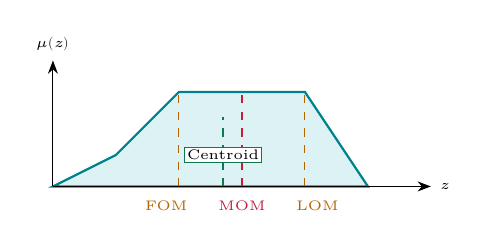
\begin{tikzpicture}[scale=0.8, every node/.style={font=\tiny}]
  % Shape
  \draw[thick, fill=hdrteal, draw=myteal] (0,0) -- (1,0.5) -- (2,1.5) -- (4,1.5) -- (5,0) -- cycle;
  \draw[-Stealth] (0,0) -- (6,0) node[right] {$z$};
  \draw[-Stealth] (0,0) -- (0,2.0) node[above] {$\mu(z)$};

  % MOM
  \draw[dashed, thick, color=myred] (3, 0) -- (3, 1.5);
  \node at (3, -0.3) [color=myred] {MOM};

  % FOM
  \draw[dashed, color=myamber] (2, 0) -- (2, 1.5);
  \node at (1.8, -0.3) [color=myamber] {FOM};

  % LOM
  \draw[dashed, color=myamber] (4, 0) -- (4, 1.5);
  \node at (4.2, -0.3) [color=myamber] {LOM};

  % Centroid
  \draw[dashed, thick, color=mygreen] (2.7, 0) -- (2.7, 1.1);
  \node at (2.7, 0.5) [draw=mygreen, fill=white, inner sep=1pt] {Centroid};
\end{tikzpicture}
\end{tcolorbox}

% ===============================================================================
\section{Lambda Cuts (\texorpdfstring{$\lambda$}{lambda}-cuts)}
% ===============================================================================

A $\lambda$-cut (or $\alpha$-cut) operation converts a fuzzy set or fuzzy relation into a classical (crisp) set by thresholding.

\begin{tcolorbox}[defbox, title={Lambda Cut ($\lambda$-cut)}]
The $\lambda$-cut of a fuzzy set $A$, denoted by $A_{\lambda}$, is a crisp set containing all elements whose membership values are greater than or equal to $\lambda$:
\begin{equation}
  A_{\lambda} = \left\{ x \in U \mid \mu_A(x) \ge \lambda \right\} \quad \text{where } \lambda \in [0, 1]
\end{equation}
\end{tcolorbox}

% ===============================================================================
\section{Worked Examples}
% ===============================================================================

\begin{tcolorbox}[examplebox, title={Fuzzy Set Operations}]
\textbf{Problem:} Given two discrete fuzzy sets defined on $U = \{1, 2, 3, 4\}$:
\begin{equation*}
  A = \left\{ \frac{0.2}{1}, \frac{0.7}{2}, \frac{1.0}{3}, \frac{0.4}{4} \right\}, \quad B = \left\{ \frac{0.5}{1}, \frac{0.6}{2}, \frac{0.3}{3}, \frac{0.9}{4} \right\}
\end{equation*}
Calculate: (a) $A \cup B$, (b) $A \cap B$, and (c) the algebraic product $A \cdot B$.
\par\vspace{4pt}\noindent\rule{\linewidth}{0.5pt}\par
\textbf{Solution:}
Recall: $\mu_{A \cup B} = \max(\mu_A, \mu_B)$, $\mu_{A \cap B} = \min(\mu_A, \mu_B)$, and $\mu_{A \cdot B} = \mu_A \cdot \mu_B$.
\par\vspace{4pt}
\begin{itemize}[leftmargin=*, itemsep=3.5pt]
  \item \textbf{(a) Union ($A \cup B$):}
    \begin{align*}
      \mu_{A \cup B}(1) &= \max(0.2, 0.5) = 0.5 \\
      \mu_{A \cup B}(2) &= \max(0.7, 0.6) = 0.7 \\
      \mu_{A \cup B}(3) &= \max(1.0, 0.3) = 1.0 \\
      \mu_{A \cup B}(4) &= \max(0.4, 0.9) = 0.9 \\
      A \cup B &= \left\{ \frac{0.5}{1}, \frac{0.7}{2}, \frac{1.0}{3}, \frac{0.9}{4} \right\}
    \end{align*}
  \item \textbf{(b) Intersection ($A \cap B$):}
    \begin{align*}
      A \cap B &= \left\{ \frac{\min(0.2,0.5)}{1}, \frac{\min(0.7,0.6)}{2}, \frac{\min(1.0,0.3)}{3}, \frac{\min(0.4,0.9)}{4} \right\} \\
      &= \left\{ \frac{0.2}{1}, \frac{0.6}{2}, \frac{0.3}{3}, \frac{0.4}{4} \right\}
    \end{align*}
  \item \textbf{(c) Algebraic Product ($A \cdot B$):}
    \begin{align*}
      A \cdot B &= \left\{ \frac{0.2 \times 0.5}{1}, \frac{0.7 \times 0.6}{2}, \frac{1.0 \times 0.3}{3}, \frac{0.4 \times 0.9}{4} \right\} \\
      &= \left\{ \frac{0.10}{1}, \frac{0.42}{2}, \frac{0.30}{3}, \frac{0.36}{4} \right\}
    \end{align*}
\end{itemize}
\end{tcolorbox}

\begin{tcolorbox}[examplebox, title={Max-Min Composition of Fuzzy Relations}]
\textbf{Problem:} Given fuzzy relations $R$ (size $2 \times 2$) and $S$ (size $2 \times 2$):
\begin{equation*}
  R = \begin{bmatrix} 0.6 & 0.3 \\ 0.2 & 0.9 \end{bmatrix}, \quad S = \begin{bmatrix} 0.5 & 0.8 \\ 0.7 & 0.1 \end{bmatrix}
\end{equation*}
Compute the Max-Min composition $T = R \circ S$.
\par\vspace{4pt}\noindent\rule{\linewidth}{0.5pt}\par
\textbf{Solution:}
The formulation is $t_{ik} = \max_j \left\{ \min\left(r_{ij}, s_{jk}\right) \right\}$.
\begin{itemize}[leftmargin=*, itemsep=3.5pt]
  \item \textbf{Element $t_{11}$:}
    \begin{equation*}
      t_{11} = \max\left( \min(0.6, 0.5), \min(0.3, 0.7) \right) = \max(0.5, 0.3) = 0.5
    \end{equation*}
  \item \textbf{Element $t_{12}$:}
    \begin{equation*}
      t_{12} = \max\left( \min(0.6, 0.8), \min(0.3, 0.1) \right) = \max(0.6, 0.1) = 0.6
    \end{equation*}
  \item \textbf{Element $t_{21}$:}
    \begin{equation*}
      t_{21} = \max\left( \min(0.2, 0.5), \min(0.9, 0.7) \right) = \max(0.2, 0.7) = 0.7
    \end{equation*}
  \item \textbf{Element $t_{22}$:}
    \begin{equation*}
      t_{22} = \max\left( \min(0.2, 0.8), \min(0.9, 0.1) \right) = \max(0.2, 0.1) = 0.2
    \end{equation*}
\end{itemize}
Thus, the composition is:
\begin{equation*}
  T = R \circ S = \begin{bmatrix} 0.5 & 0.6 \\ 0.7 & 0.2 \end{bmatrix}
\end{equation*}
\end{tcolorbox}

\begin{tcolorbox}[examplebox, title={Discrete Centroid Defuzzification}]
\textbf{Problem:} Calculate the crisp value $z^*$ of the fuzzy set $C$ using Centroid defuzzification:
\begin{equation*}
  C = \left\{ \frac{0.1}{10}, \frac{0.3}{20}, \frac{0.8}{30}, \frac{1.0}{40}, \frac{0.6}{50} \right\}
\end{equation*}
\par\vspace{4pt}\noindent\rule{\linewidth}{0.5pt}\par
\textbf{Solution:}
We use the discrete Centroid formula: $z^* = \frac{\sum z_i \mu_C(z_i)}{\sum \mu_C(z_i)}$.
\par\vspace{4pt}
\begin{align*}
  \sum z_i \mu_C(z_i) &= 10(0.1) + 20(0.3) + 30(0.8) + 40(1.0) + 50(0.6) \\
  &= 1 + 6 + 24 + 40 + 30 = 101 \\
  \sum \mu_C(z_i) &= 0.1 + 0.3 + 0.8 + 1.0 + 0.6 = 2.8 \\
  z^* &= \frac{101}{2.8} \approx 36.07
\end{align*}
The defuzzified crisp output is $z^* \approx 36.07$.
\end{tcolorbox}

\newpage

% ===============================================================================
% MANDATORY QUICK REVISION PAGE
% ===============================================================================
\begin{center}
  {\large\bfseries\color{myred} Quick Revision --- Module IV}\\[3pt]
  {\small\color{mydark} Fuzzy Sets and Membership Functions $|$ PE-EC702C}
\end{center}
\noindent{\color{myred}\rule{\linewidth}{1.2pt}}
\vspace{4pt}

\begin{tcolorbox}[formulabox, title={\textbf{Key Formulas at a Glance}}]
\renewcommand{\arraystretch}{1.3}
\begin{tabularx}{\linewidth}{B{5.0cm} X}Fuzzy Union (OR) & $\mu_{A \cup B}(x) = \max(\mu_A(x), \mu_B(x))$ \\
Fuzzy Intersection (AND) & $\mu_{A \cap B}(x) = \min(\mu_A(x), \mu_B(x))$ \\
Max-Min Composition & $\mu_{R \circ S}(x, z) = \max_y \{ \min( \mu_R(x,y), \mu_S(y,z) ) \}$ \\
Max-Product Composition & $\mu_{R \bullet S}(x, z) = \max_y \{ \mu_R(x,y) \cdot \mu_S(y,z) \}$ \\
Centroid Defuzzification & $z^* = \frac{\sum z_i \mu_C(z_i)}{\sum \mu_C(z_i)} \quad \text{or} \quad \frac{\int z \mu_C(z) dz}{\int \mu_C(z) dz}$ \\
Lambda-Cut ($\lambda$-cut) & $A_{\lambda} = \{ x \in U \mid \mu_A(x) \ge \lambda \}$
\end{tabularx}
\tcbset{colbacktitle=myteal, coltitle=white}
\end{tcolorbox}

\begin{tcolorbox}[defbox, title={\textbf{One-Line Definitions}}]
\begin{itemize}[leftmargin=*, itemsep=2.5pt, topsep=0pt]
  \item \textbf{Fuzzy Set:} A set containing elements with varying degrees of membership represented by values in $[0, 1]$.
  \item \textbf{Membership Function:} The graphical curve or mathematical function that maps elements to their membership degrees.
  \item \textbf{Centroid Defuzzification:} A defuzzification method that calculates the center of gravity of the output fuzzy region.
  \item \textbf{Lambda Cut:} An operation that converts a fuzzy set/relation into a classical set using a threshold value $\lambda$.
  \item \textbf{Crossover Point:} Any element in the universe of discourse whose membership degree in a fuzzy set is exactly $0.5$.
\end{itemize}
\tcbset{colbacktitle=myteal, coltitle=white}
\end{tcolorbox}

\begin{tcolorbox}[exambox, title={\textbf{Frequently Asked / Viva Questions}}]
\begin{enumerate}[leftmargin=*, itemsep=3.5pt, label=\arabic*.]
  \item \Q{What is the difference between probability and fuzziness?} Probability deals with the likelihood/chance of an event occurring (undecided outcome). Fuzziness deals with the vagueness of an event that has already occurred (deterministic but vague boundaries, e.g. "He is tall").
  \item \Q{State the properties of classical sets that do NOT hold in fuzzy sets.} The Law of Contradiction ($A \cap \bar{A} = \emptyset$) and the Law of Excluded Middle ($A \cup \bar{A} = U$) do not hold in fuzzy sets (e.g. $A \cap \bar{A} \neq \emptyset$).
  \item \Q{What is a normal fuzzy set?} A fuzzy set is normal if its height is exactly $1.0$ (i.e. at least one element has a membership value of $1$).
  \item \Q{Define a subnormal fuzzy set.} A fuzzy set whose maximum membership value (height) is strictly less than $1.0$.
  \item \Q{Why is Centroid defuzzification the most commonly used method?} Because it integrates the entire area of the output fuzzy shape, yielding smooth, continuous output transitions relative to changes in inputs.
  \item \Q{Explain the Max-Min composition rule.} It is a method of relating elements of set $X$ to set $Z$ through intermediate set $Y$. For each $(x,z)$ pair, it finds the strength of paths through all $y \in Y$ (using Min) and selects the strongest path (using Max).
  \item \Q{What is the difference between a tolerance relation and an equivalence relation?} An equivalence relation must be reflexive, symmetric, and transitive. A tolerance relation is only reflexive and symmetric (not transitive).
  \item \Q{Define the support of a fuzzy set.} The crisp set of all elements in the universe of discourse whose membership values are strictly greater than $0$ ($\mu_A(x) > 0$).
  \item \Q{What are the standard forms of membership functions?} Triangular, Trapezoidal, Gaussian, Sigmoidal, L-shaped, and S-shaped curves.
  \item \Q{What is the purpose of defuzzification in fuzzy controllers?} Physical actuators and microcontrollers require crisp, exact values (like voltage or valve position) to operate, which requires defuzzification of the fuzzy control decision.
\end{enumerate}
\tcbset{colbacktitle=myteal, coltitle=white}
\end{tcolorbox}

\begin{tcolorbox}[tikzbox, title={Crisp Sets vs. Fuzzy Sets}]
\centering
{\renewcommand{\arraystretch}{1.55}%
\begin{tabularx}{\linewidth}{|>{\bfseries}B{3.2cm}|Y|Y|}
\hline
Attribute & Classical (Crisp) Sets & Fuzzy Sets \\
\hline
Membership Values & Binary: $\{0, 1\}$ & Continuous: $[0, 1]$ \\
\hline
Boundaries & Sharp, distinct boundaries & Gradual, vague boundaries \\
\hline
Operations & Boolean logic (AND, OR, NOT) & Fuzzy logic (Min, Max, $1-\mu$) \\
\hline
Contradiction Law & Holds: $A \cap \bar{A} = \emptyset$ & Does not hold: $A \cap \bar{A} \neq \emptyset$ \\[4pt]
\hline
\end{tabularx}}
\tcbset{colbacktitle=myteal, coltitle=white}
\end{tcolorbox}


% -- Module 5 -----------------------------------------------------------------
\modulestart{5}{Applications of Artificial Neural Networks}

\section{Applications of Artificial Neural Networks}
% ===============================================================================

Neural networks excel at pattern recognition, function approximation, and adaptive modeling due to their parallel distributed architecture and learning capabilities.

\begin{enumerate}[leftmargin=*, itemsep=4pt]
  \item \textbf{Pattern and Character Recognition:} ANNs (particularly CNNs and MLPs) are widely used for Optical Character Recognition (OCR), signature verification, and face recognition by learning translation-invariant spatial features.
  \item \textbf{Image Compression:} Feedforward networks with a narrow hidden layer (bottleneck autoencoders) perform dimensionality reduction. The input image is reconstructed at the output layer, while the compressed representation is stored at the hidden layer.
  \item \textbf{Communication Systems (Channel Equalization):} Equalizers modeled using neural networks (like radial basis function networks) reduce Inter-Symbol Interference (ISI) in dispersive channels by acting as non-linear classifiers.
  \item \textbf{Control Systems (System Identification):} ANNs model the forward and inverse dynamics of complex, non-linear chemical and mechanical processes, facilitating adaptive and predictive control schemes.
\end{enumerate}

% ===============================================================================
\section{Applications of Fuzzy Logic}
% ===============================================================================

Fuzzy logic is highly effective in systems involving linguistic variables and human decision-making processes, where exact mathematical models are unavailable.

\begin{itemize}[leftmargin=*, itemsep=3pt]
  \item \textbf{Fuzzy Pattern Recognition:} Classifies inputs into overlapping classes based on membership values rather than crisp thresholds.
  \item \textbf{Fuzzy Image Compression:} Uses fuzzy rules to adaptively select quantization levels across different image blocks based on local edge/texture complexity.
\end{itemize}

% ===============================================================================
\section{Fuzzy Logic Controllers (FLC)}
% ===============================================================================

A Fuzzy Logic Controller (FLC) implements a control algorithm by evaluating heuristic, rule-based statements rather than mathematical differential equations.

\begin{tcolorbox}[tikzbox, title={Fuzzy Logic Controller Block Diagram}]
\centering
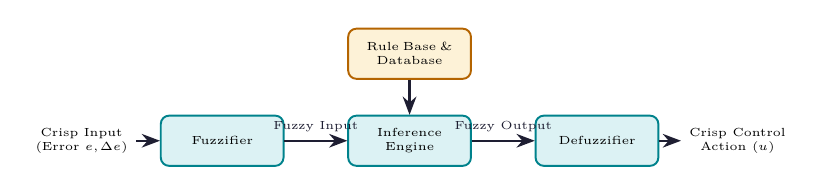
\begin{tikzpicture}[scale=0.85, every node/.style={transform shape, font=\tiny},
  block/.style={rectangle, draw=myteal, fill=hdrteal,
    text width=1.6cm, align=center, minimum height=0.75cm,
    font=\tiny, rounded corners=3pt, line width=0.7pt}]
  
  % Blocks
  \node[block] (fuzz) at (0, 0) {Fuzzifier};
  \node[block] (infer) at (2.8, 0) {Inference\\Engine};
  \node[block] (defuzz) at (5.6, 0) {Defuzzifier};
  
  \node[block, draw=myamber, fill=hdramber] (rules) at (2.8, 1.3) {Rule Base \&\\Database};

  % Inputs & Outputs
  \node (in) at (-2.1, 0) [align=center, font=\fontsize{5}{6}\selectfont] {Crisp Input\\(Error $e, \Delta e$)};
  \node (out) at (7.7, 0) [align=center, font=\fontsize{5}{6}\selectfont] {Crisp Control\\Action ($u$)};

  % Connections
  \draw[arrow] (in) -- (fuzz);
  \draw[arrow] (fuzz) -- node[midway, above, font=\fontsize{5}{6}\selectfont\color{myteal}] {Fuzzy Input} (infer);
  \draw[arrow] (infer) -- node[midway, above, font=\fontsize{5}{6}\selectfont\color{myteal}] {Fuzzy Output} (defuzz);
  \draw[arrow] (defuzz) -- (out);
  
  \draw[arrow] (rules.south) -- (infer.north);
\end{tikzpicture}
\end{tcolorbox}

\subsection{Standard FLC Architecture Components}
\begin{enumerate}[leftmargin=*, itemsep=3.5pt]
  \item \textbf{Fuzzifier (Fuzzification Interface):} Measures physical inputs and converts them into fuzzy values (linguistic terms like *Positive Big*, *Zero*, *Negative Small*) using predefined input membership functions.
  \item \textbf{Knowledge Base (Rule \& Database):} Contains the database (definitions of membership functions) and the Rule Base (a collection of linguistic control statements in \textbf{IF-THEN} format).
  \item \textbf{Inference Engine (Decision Making Logic):} Evaluates the active rules to determine the overall fuzzy control output based on composition rules (usually Max-Min composition).
  \item \textbf{Defuzzifier (Defuzzification Interface):} Converts the combined fuzzy output into a single crisp control command to drive physical actuators.
\end{enumerate}

% ===============================================================================
\section{Control System Case Studies}
% ===============================================================================

\subsection{Inverted Pendulum Controller}
The goal is to maintain a rotating pole in an upright position by moving a motorized cart horizontally.

\begin{tcolorbox}[tikzbox, title={Inverted Pendulum Physical Model}]
\centering
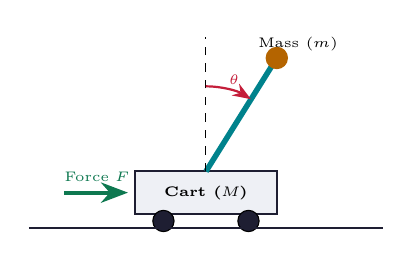
\begin{tikzpicture}[scale=0.9, every node/.style={font=\tiny}]
  % Cart
  \draw[thick, fill=hdrgray, draw=mydark] (-1, 0) rectangle (1, 0.6);
  \draw[fill=mydark] (-0.6, -0.1) circle (0.15);
  \draw[fill=mydark] (0.6, -0.1) circle (0.15);
  \node at (0, 0.3) {\textbf{Cart ($M$)}};

  % Ground
  \draw[line] (-2.5, -0.2) -- (2.5, -0.2);

  % Pendulum Pole
  \draw[line, line width=2pt, color=myteal] (0, 0.6) -- (1.0, 2.2);
  \draw[fill=myamber, draw=myamber] (1.0, 2.2) circle (0.15);
  \node at (1.3, 2.4) {Mass ($m$)};
  
  % Angle
  \draw[dashed] (0, 0.6) -- (0, 2.5);
  \draw[arrow, color=myred] (0, 1.8) arc (90:58:1.2);
  \node at (0.4, 1.9) [color=myred] {$\theta$};

  % Force arrow
  \draw[arrow, line width=1.5pt, color=mygreen] (-2.0, 0.3) -- (-1.1, 0.3) node[midway, above] {Force $F$};
\end{tikzpicture}
\end{tcolorbox}

\par\noindent
\begin{itemize}[leftmargin=*, itemsep=3pt]
  \item \textbf{Inputs:} Angle error $\theta$ (deviation from vertical) and angular velocity $e_{\omega} = d\theta/dt$.
  \item \textbf{Output:} Motor force $F$ applied to the cart.
  \item \textbf{Rule Base example:}
    \begin{itemize}[leftmargin=1.5em]
      \item \textit{IF angle ($\theta$) is Positive Small AND angular velocity ($d\theta/dt$) is Zero, THEN force ($F$) is Positive Small.}
    \end{itemize}
\end{itemize}

\subsection{Fuzzy Washing Machine Controller}
An FLC optimizes the wash cycle time, water temperature, and spin speed based on:
\begin{itemize}[leftmargin=*, itemsep=3pt]
  \item \textbf{Inputs:} Dirtiness level of clothes (using optical sensors that measure water transparency) and weight of load.
  \item \textbf{Output:} Cycle duration (wash time).
  \item \textbf{Rule Base example:}
    \begin{itemize}[leftmargin=1.5em]
      \item \textit{IF dirtiness is High AND weight is Medium, THEN wash time is Long.}
    \end{itemize}
\end{itemize}

% ===============================================================================
\section{Worked Examples}
% ===============================================================================

\begin{tcolorbox}[examplebox, title={Fuzzy Inference System Evaluation}]
\textbf{Problem:} Consider a simple Fuzzy Logic Controller with two input variables $x$ (error) and $y$ (change of error), and one output $z$ (control force).
The fuzzy rule base contains the following two rules:
\begin{itemize}[leftmargin=*, itemsep=2pt]
  \item \textbf{Rule 1:} IF $x$ is $A_1$ AND $y$ is $B_1$, THEN $z$ is $C_1$
  \item \textbf{Rule 2:} IF $x$ is $A_2$ AND $y$ is $B_2$, THEN $z$ is $C_2$
\end{itemize}

Given crisp input values $x_0 = 4$ and $y_0 = 6$:
\begin{itemize}[leftmargin=*, itemsep=2pt]
  \item Membership values: $\mu_{A_1}(x_0) = 0.6, \quad \mu_{A_2}(x_0) = 0.3, \quad \mu_{B_1}(y_0) = 0.8, \quad \mu_{B_2}(y_0) = 0.4$
  \item Output membership centers (represented by singletons): $z_{C_1} = 20, \quad z_{C_2} = 50$
\end{itemize}
Evaluate the output control value $z^*$ using the \textbf{weighted average} defuzzification method.
\par\vspace{4pt}\noindent\rule{\linewidth}{0.5pt}\par
\textbf{Solution:}

\textbf{1. Compute Firing Strengths ($\alpha$-levels) of the rules:}
Since the connective is \textbf{AND}, we use the Min operator:
\begin{itemize}[leftmargin=*, itemsep=2.5pt]
  \item For \textbf{Rule 1}:
    \begin{equation*}
      \alpha_1 = \min\left( \mu_{A_1}(x_0), \mu_{B_1}(y_0) \right) = \min(0.6, 0.8) = 0.6
    \end{equation*}
  \item For \textbf{Rule 2}:
    \begin{equation*}
      \alpha_2 = \min\left( \mu_{A_2}(x_0), \mu_{B_2}(y_0) \right) = \min(0.3, 0.4) = 0.3
    \end{equation*}
\end{itemize}

\par\vspace{4pt}
\textbf{2. Calculate Defuzzified Output ($z^*$):}
Using the weighted average formula:
\begin{align*}
  z^* &= \frac{\alpha_1 z_{C_1} + \alpha_2 z_{C_2}}{\alpha_1 + \alpha_2} \\
  &= \frac{0.6(20) + 0.3(50)}{0.6 + 0.3} \\
  &= \frac{12 + 15}{0.9} = \frac{27}{0.9} = 30
\end{align*}
The output control force is $z^* = 30$.
\end{tcolorbox}

\newpage

% ===============================================================================
% MANDATORY QUICK REVISION PAGE
% ===============================================================================
\begin{center}
  {\large\bfseries\color{myred} Quick Revision --- Module V}\\[3pt]
  {\small\color{mydark} Applications of Neural Networks \& Fuzzy Logic $|$ PE-EC702C}
\end{center}
\noindent{\color{myred}\rule{\linewidth}{1.2pt}}
\vspace{4pt}

\begin{tcolorbox}[formulabox, title={\textbf{Key Formulas at a Glance}}]
\renewcommand{\arraystretch}{1.3}
\begin{tabularx}{\linewidth}{B{5.0cm} X}Rule Firing Strength (AND) & $\alpha_i = \min\left( \mu_{A_i}(x_0), \mu_{B_i}(y_0) \right)$ \\
Rule Firing Strength (OR) & $\alpha_i = \max\left( \mu_{A_i}(x_0), \mu_{B_i}(y_0) \right)$ \\
Weighted Average Defuzzification & $z^* = \frac{\sum \alpha_i z_i}{\sum \alpha_i}$ \\
Inverted Pendulum Angle Error & $e(t) = \theta_{ref} - \theta(t)$ \\
Inverted Pendulum Error Change & $\Delta e(t) = e(t) - e(t-1)$
\end{tabularx}
\tcbset{colbacktitle=myteal, coltitle=white}
\end{tcolorbox}

\begin{tcolorbox}[defbox, title={\textbf{One-Line Definitions}}]
\begin{itemize}[leftmargin=*, itemsep=2.5pt, topsep=0pt]
  \item \textbf{Fuzzy Controller:} A control device that uses linguistic rules and fuzzy reasoning to calculate system control inputs.
  \item \textbf{Fuzzifier:} The interface in an FLC that maps physical crisp sensor readings to linguistic fuzzy values.
  \item \textbf{Inference Engine:} The decision-making unit that evaluates active rule statements to determine control signals.
  \item \textbf{Linguistic Variable:} A variable whose values are words or sentences in a language rather than numbers (e.g. "Warm").
  \item \textbf{System Identification:} The process of developing a mathematical or neural network model to describe dynamic process behavior.
\end{itemize}
\tcbset{colbacktitle=myteal, coltitle=white}
\end{tcolorbox}

\begin{tcolorbox}[exambox, title={\textbf{Frequently Asked / Viva Questions}}]
\begin{enumerate}[leftmargin=*, itemsep=3.5pt, label=\arabic*.]
  \item \Q{What are the main advantages of a Fuzzy Logic Controller over a PID controller?} FLCs do not require an exact mathematical model of the process, can handle non-linear dynamics easily, and can incorporate human operator heuristics directly using linguistic rules.
  \item \Q{State the function of the FLC Rule Base.} The Rule Base contains the control logic written as a set of IF-THEN rules that describe the relationship between input error conditions and output control actions.
  \item \Q{How is a neural network used for image compression?} An autoencoder network is trained to replicate inputs at its output layer. A bottleneck hidden layer (fewer nodes) forces the network to learn a compressed representation of the image.
  \item \Q{What is channel equalization in communications, and how do ANNs help?} Channel equalization compensates for signal distortion (ISI) caused by transmission channels. ANNs act as adaptive classifiers that identify non-linear decision boundaries to recover transmitted symbols.
  \item \Q{Explain the wash time optimization in a fuzzy washing machine.} Sensors measure the quantity of load and the dirtiness of the water (transparency). The FLC infers the optimum wash cycle time: muddy water with a heavy load triggers a long wash cycle.
  \item \Q{What inputs are required to balance an inverted pendulum?} The deviation angle $\theta$ from the vertical axis (error) and the rate of change of the angle $d\theta/dt$ (angular velocity).
  \item \Q{What is the difference between Mamdani and Sugeno fuzzy inference systems?} Mamdani systems use fuzzy sets for output membership functions, requiring defuzzification. Sugeno systems use linear mathematical functions or constants for outputs, simplifying calculation.
  \item \Q{Define a Singleton membership function.} A singleton is a membership function that has a value of $1.0$ at a single specific point and $0$ everywhere else.
  \item \Q{How does a neural network model non-linear control systems?} By acting as a system identification model, learning the mapping between system input history and corresponding output responses.
  \item \Q{What is the role of the database in a fuzzy controller?} The database holds the exact parameters (shapes, coordinates, limits) of the membership functions defined for the input and output variables.
\end{enumerate}
\tcbset{colbacktitle=myteal, coltitle=white}
\end{tcolorbox}

\begin{tcolorbox}[tikzbox, title={Comparison of Control Strategies}]
\centering
{\renewcommand{\arraystretch}{1.55}%
\begin{tabularx}{\linewidth}{|>{\bfseries}B{3.2cm}|Y|Y|}
\hline
Parameter & Classical PID Control & Fuzzy Logic Control \\
\hline
Process Model & Requires exact mathematical model & No mathematical model required \\
\hline
Control Logic & Defined by differential equations & Defined by linguistic IF-THEN rules \\
\hline
Tuning Parameters & Proportional, Integral, Derivative gains & Membership functions and rule parameters \\[4pt]
\hline
Non-linear Handling & Difficult (often requires linearization) & Inherently handles non-linearities \\[4pt]
\hline
\end{tabularx}}
\tcbset{colbacktitle=myteal, coltitle=white}
\end{tcolorbox}


\end{document}
